\documentclass[10pt,conference]{IEEEtran}
\usepackage{cite}
\usepackage{amsmath}
\usepackage[T1]{fontenc}
\usepackage{graphicx}
\usepackage{url}
\usepackage{hyperref}
\usepackage{booktabs}
\usepackage{tabularx}
\usepackage{array}
\begin{document}
\title{A Common Standard for Comparing Reviews of Artificial Intelligence Benchmarks}
\author{Anonymous authors}
\maketitle
\begin{abstract}
\textbf{Background:} At least seven frameworks have been proposed for reviewing artificial intelligence benchmarks. They ask overlapping questions on different scales and treat undocumented items differently, and to our knowledge no two have been applied to the same benchmark at item level.
\textbf{Objective:} We introduce MESA, a standard for comparing benchmark reviews, use it to compare seven of those frameworks, and build from its shared criteria the MESA rubric, a single review form that brings the frameworks' questions together, which we then evaluate.
\textbf{Method:} Every item of the seven frameworks was mapped to a list of shared criteria. Coding agents applied each applicable framework to fixed snapshots of four benchmarks, and every answer was recoded as met, not met or open, with a label on negative scores that follow only from something the benchmark does not report. The MESA rubric was applied twice per benchmark, and an assistant model checked every rating against its cited sources.
\textbf{Results:} No criterion is asked by all seven frameworks, and five penalize undocumented items by design. Framework pairs agree on about half of the criteria they share: on documentation and licensing, rarely on validity. Under this mapping and agent setup, the disagreements are consistent with differences in framework design, in how finely a framework splits a criterion and in its rule for undocumented items, rather than with different readings of the sources. Negative answers given because the benchmark does not report something outnumber answers that found an actual problem by more than ten to one, although the first group mixes missing reports with practices that may exist unreported. The MESA rubric gives the same rating on four repeats in five, records undocumented items as open questions rather than failures, and most of its ratings held up when checked against the sources they cite.
\textbf{Conclusion:} MESA gives benchmark reviews what they lacked, a shared vocabulary that lets frameworks be compared on the same benchmark and a way to tell an actual problem from something the benchmark simply does not report. With it, the disagreements between frameworks in this study could be traced to their design rather than to different readings of the evidence, and the rubric built on it gave ratings that can be checked against the sources they cite. Checking those ratings with human reviewers is the next step.
\end{abstract}
\begin{IEEEkeywords}
benchmark review, measurement, evaluation frameworks, coding agents, evidence, software evaluation
\end{IEEEkeywords}

\section{Introduction}
Suppose a research team wants to know whether a widely used artificial intelligence benchmark can be trusted before relying on its scores. They look for a review of the benchmark, or sit down to write one, and discover that since 2023 at least seven review frameworks have been published for that job \cite{cohn_hernandez_orallo_oecd_2023,reuel_betterbench,liu_ecbd_2024,cao_how2bench_2025,zhu_agentic_benchmark_checklist_2025,san_joaquin_scorecard_2026,corona_benchmark_caliper_2026}. Each framework asks sensible questions about a measuring instrument: whether its tasks capture the ability it claims to test, whether its reference answers and grading scripts work as described, whether another team can repeat the evaluation, and whether the scores support the conclusions drawn from them. Yet if our team picks two frameworks and applies both to the same benchmark, they run into an immediate obstacle. The frameworks do not speak the same language.

Consider a concrete question that every careful reviewer asks: did the benchmark creators check whether their test material appeared in the training data of the models they evaluated, or take steps to guard against contamination? BetterBench asks two implementation questions about unique identifiers, encryption and contamination tasks, scoring each 0, 5, 10 or 15, and gives 0 whenever the paper and repository do not mention the item \cite{reuel_betterbench}. How2Bench asks a single construction question and labels a benchmark as not considering contamination unless the paper gives explicit textual evidence \cite{cao_how2bench_2025}. The Scorecard of AI Benchmark Quality asks under internal validity (whether scores are free of confounding flaws) whether the evaluated model and any judge model were trained on overlapping data, marking the item satisfied or unsatisfied \cite{san_joaquin_scorecard_2026}. The Agentic Benchmark Checklist asks under reporting whether the benchmark includes a private test set or an update plan, scoring 1 or 0 \cite{zhu_agentic_benchmark_checklist_2025}. Meanwhile, the Evidence Centered Benchmark Design (ECBD) worksheet, Benchmark Caliper and the 18-facet OECD classification framework do not ask about training data overlap at all \cite{liu_ecbd_2024,corona_benchmark_caliper_2026,cohn_hernandez_orallo_oecd_2023}. When a benchmark paper simply says nothing about training data overlap, four frameworks turn that missing statement into a low score or a failure, while three say nothing. A reader looking at the resulting outputs cannot tell where the frameworks agree, where they disagree about the evidence in the benchmark, and where they merely follow opposite rule for undocumented items.

Evidence-based medicine treats its study appraisal tools as instruments to be tested. When Hartling et al.\ tested the Cochrane risk-of-bias tool on randomized trials and the Newcastle-Ottawa scale on cohort studies, each with independent reviewers, they found agreement between reviewers low enough to conclude that the tools need more specific guidance to be applied consistently \cite{hartling_rand_2012}. The lesson we take is a modest one: an appraisal instrument is examined by applying it and tracing its disagreements, and those disagreements often lead back to the instrument's wording and guidance rather than to the studies. Benchmark review in artificial intelligence has no equivalent body of comparisons, even as new checklists and scorecards continue to appear every few months.

We introduce MESA, the Meta-Evaluation Standard for AI, to provide the common vocabulary that makes such comparisons possible. MESA is not an eighth disconnected checklist; it is a translation layer and review standard built from the existing seven frameworks. It has four parts:
\begin{enumerate}
\item A list of 30 shared review criteria onto which every item of the seven frameworks (280 items in all) is mapped.
\item Three common verdicts per criterion (\emph{met}, \emph{not met} and \emph{open}) into which any framework's answer scale is recoded, paired with explicit qualifiers that preserve partial fulfillment and distinguish problems the sources show from negative scores caused by undocumented items.
\item A structured answer record for each answer and rating carrying the reviewer's reason, source document identifiers, line or page locators, verbatim quotes, a note on what information was missing, and the checks performed.
\item A descriptive profile of the benchmark, recorded before evaluation using the eight OECD facets with high rater agreement \cite{cohn_hernandez_orallo_oecd_2023}, which determines which evaluation criteria apply to a given instrument.
\end{enumerate}

We use MESA in a two-part study across four benchmarks that span different tasks: HumanEval, in which a model writes Python functions from docstrings and is scored by unit tests \cite{human_eval_repository}; TruthfulQA, a set of questions designed to elicit common human falsehoods, scored for truthfulness and informativeness \cite{truthfulqa_repository}; Humanity's Last Exam, a collection of expert written academic questions at the frontier of model ability \cite{phan_etal_hle_2025}; and $\tau$-bench, in which an agent serves simulated airline and retail customers through tools and a policy document \cite{tau_bench_repository}. In Study 1, coding agents apply each applicable existing framework to fixed snapshots of the benchmarks' papers and repositories, and MESA recodes both the agents' answers and the framework authors' own published reviews onto the 30 criteria. Comparing the agent's BetterBench ratings against the BetterBench authors' published ratings on HumanEval and TruthfulQA serves as a proof of concept that an agent given a framework's verbatim items and guidance lands near the framework's creators. In Study 2, we evaluate the MESA rubric that puts the standard into practice: a description part, Description (Part A, eight facets that record what kind of instrument the benchmark is before any rating) followed by an evaluation part, Evaluation (Part B, 29 evaluation questions, one per criterion), each question rated with positive levels that separate an unverified claim (\emph{Claimed}) from an inspectable artifact (\emph{Documented}) and a documented verification (\emph{Verified}), alongside a single defect level (\emph{Contradicted}) and two null states (\emph{Undocumented} and \emph{Not applicable}). The MESA rubric was derived from the finalized mapping and the frameworks' item specifications before any agent session ran, so Study 1 empirical verdicts do not shape it.

We organize the investigation around four research questions:
\begin{itemize}
\item \textbf{RQ1.} Which criteria do existing benchmark review frameworks cover?
\item \textbf{RQ2.} Do the frameworks agree when applied to the same benchmark?
\item \textbf{RQ3.} How does each framework treat information that a benchmark does not report?
\item \textbf{RQ4.} When a rubric is derived from the existing frameworks, do its ratings hold up when the cited sources are checked?
\end{itemize}

This paper makes five contributions: (1) the MESA standard (30 shared criteria, three recoded verdicts with qualifiers, structured evidence records and pre-evaluation description); (2) the complete mapping of 280 items across seven frameworks to the 30 criteria, recording the assistant model's initial draft, the author's independent mapping and every reconciliation note; (3) the structural analysis of coverage, answerability and rule for undocumented items across all seven frameworks, together with the recoded baseline of published reviews; (4) the MESA rubric, eight facets and 29 questions with full item lineage and the two-study evaluation protocol; and (5) empirical findings from 28 coding agent sessions and 296 source-checked rubric ratings across four benchmarks.

\section{Background and Related Work}
Our work sits at the intersection of four areas: measurement standards from psychology and education, the seven frameworks proposed for reviewing artificial intelligence benchmarks, automated auditors that inspect individual benchmark tasks, and comparative reliability studies of appraisal tools in medicine.

\subsection{Test review and score validity}
In educational and psychological measurement, validity is not a static property of a test; it is the degree to which evidence and theory support the interpretation and use of test scores for a stated purpose \cite{kane_validation,aera_apa_ncme_standards_2014}. Turning that principle into a practical review of a test requires separating what a test looks like from how well its evidence holds up. The 2025 version of the European Federation of Psychologists' Associations (EFPA) Test Review Model makes that separation explicit: a reviewer first completes a neutral description of the instrument (its purpose, administration, scoring mode and reference group) and only then rates its technical quality (how well its tasks represent the claimed skill or construct, how reliable its scores are, and what validity evidence supports them) using anchored scales that keep missing documentation distinct from negative evidence \cite{efpa_test_review_model_2025}.

Cohn and Hern\'andez-Orallo brought this taxonomic tradition to artificial intelligence evaluation with eighteen facets grouped under validity, consistency and fairness \cite{cohn_categorising_2022,cohn_hernandez_orallo_oecd_2023}. Each facet assigns an evaluation instrument to one of two to four categorical values. When four raters applied the eighteen facets to twenty evaluation instruments in the 2023 OECD study, a striking split emerged. On facets that describe observable design choices, such as whether scoring is manual or automated (\emph{Judgeability}) or whether the test is meant for research or conformity (\emph{Purpose}), the raters agreed consistently. On facets that require judging the quality of a benchmark's argument, such as whether its task distribution is unbiased (\emph{Coverage}) or whether scores reflect the target skill without confounds (\emph{Specificity}), raters disagreed on a third to half of the instruments \cite{cohn_hernandez_orallo_oecd_2023}. Because the OECD facets were designed to classify instruments rather than compare reviews, they have not been applied to benchmarks released after 2022, and no study has linked them to the checklists that followed.

\subsection{Frameworks for reviewing benchmarks}
Between 2023 and 2026, six additional frameworks appeared alongside the OECD facets. Table~\ref{tab:frameworks} summarizes all seven frameworks, their intended scope, the item counts stated in their papers versus what their published materials actually contain, their answer scales, the benchmarks their authors applied them to, and their role in our study.

\begin{table*}[t]
\caption{The seven review frameworks.}
\label{tab:frameworks}
\centering
\small
\begin{tabularx}{\textwidth}{@{}llrrXXX@{}}
\toprule
\textbf{Code} & \textbf{Framework} & \textbf{Items in paper} & \textbf{Items in template} & \textbf{Scope} & \textbf{Answer scale} & \textbf{Published applications and role in this study} \\
\midrule
BB & BetterBench \cite{reuel_betterbench} & 46 & 47 & General AI benchmarks across design, implementation, documentation and maintenance & 0, 5, 10, 15 or n/a per item, rolled into weighted lifecycle and overall scores & Applied by its authors to 24 benchmarks (including HumanEval and TruthfulQA). Applied in Study 1 to all four benchmarks; published reviews on HumanEval and TruthfulQA serve as proof of concept. \\
ECBD & ECBD worksheet \cite{liu_ecbd_2024} & 20 & 20 & Natural language processing benchmarks across seven modules & Free text answers arranged in describe, justify and support triples; no numerical score & Applied by its authors as case studies to SuperGLUE, BigBench and HELM. Applied in Study 1 to all four benchmarks. \\
SC & Scorecard of AI Benchmark Quality \cite{san_joaquin_scorecard_2026} & 68 & 68 & General AI benchmarks across construct, internal and external validity, reliability and correctness & 22 principles and 46 bullets marked satisfied, unsatisfied or not applicable; dimensions scored 1 to 4; suitability classes A to E & Demonstrated by two assessors on one benchmark in its paper. Applied in Study 1 to all four benchmarks. \\
H2B & How2Bench \cite{cao_how2bench_2025} & 55 & 55 & Code-related benchmarks across design, construction, evaluation, analysis and release & Checkbox per item with 1, 2 or 3 priority stars; coded present or not mentioned in the authors' survey & Used by its authors to profile 672 code benchmarks in aggregate (including HumanEval), without releasing per-benchmark item sheets. Applied in Study 1 to HumanEval. \\
ABC & Agentic Benchmark Checklist \cite{zhu_agentic_benchmark_checklist_2025} & 42 & 44 & Agentic benchmarks across task validity, outcome validity and reporting & Binary 1 (satisfied) or 0 (otherwise) per item & Applied by its authors to 10 agentic benchmarks (including 31 of 44 items on $\tau$-bench). Applied in Study 1 to $\tau$-bench; published review retained as reference data. \\
CAL & Benchmark Caliper \cite{corona_benchmark_caliper_2026} & 28 & 28 & Cultural and regional transfer across input and output ontology, content and form & 28 checklist items returning an item answer or Unknown; six dimensions scored 1 to 5 & Applied by its authors to three benchmark and region pairs (including HELM for Southeast Asia). Mapped in RQ1 for coverage; not applied in sessions because every item requires a target deployment region. \\
OECD & OECD facets \cite{cohn_hernandez_orallo_oecd_2023} & 18 & 18 & All AI evaluation instruments across validity, consistency and fairness & Categorical choice from 2 to 4 values per facet (some with free text specification; Reliability allows N/A) & Applied by four raters to 20 instruments in 2023 (reporting agreement rates but not per-instrument sheets). Applied in Study 1 to all four benchmarks; 8 high-agreement facets form Part A of the MESA rubric. \\
\bottomrule
\end{tabularx}
\par\vspace{2pt}\raggedright\footnotesize Ordered as in the mapping. Items in paper: the item count the framework's paper states; items in template: the items its released template or checklist contains, which we transcribed.
\end{table*}

The seven frameworks differ in scale, scope and rules:
\begin{itemize}
\item \textbf{BetterBench} \cite{reuel_betterbench} organizes items into design (14 items), implementation (11 items), documentation (19 items) and maintenance (3 items), scoring each 0 (not acknowledged and not addressed), 5 (acknowledged but not addressed), 10 (partially addressed), 15 (fully addressed) or n/a. Although the paper states 46 items in its prose, both its Appendix I.1 template and its public assessment database contain and score 47 distinct items; we transcribed all 47 in database order.
\item \textbf{The ECBD worksheet} \cite{liu_ecbd_2024} adapts evidence-centered design into 20 open-ended questions across seven modules (intended use, capability, content, adaptation, assembly, evidence extraction and evidence accumulation). Apart from intended use, each module asks a \emph{describe}, \emph{justify} and \emph{support} triple, recording what the benchmark creators did, why they chose it and what validity evidence they offer, without assigning numbers.
\item \textbf{The Scorecard of AI Benchmark Quality (SC, or the Scorecard)} \cite{san_joaquin_scorecard_2026} specifies 22 top-level principles and 46 subordinate bullets across five dimensions: construct validity, internal validity, external validity, reliability and correctness. Reviewers mark each item satisfied, unsatisfied or not applicable with a written justification, rate each dimension from 1 to 4 according to the severity of unsatisfied items, and assign the benchmark to a suitability class from A to E. When two of its authors independently scored the same benchmark, they disagreed on six items because they interpreted item requirements and partial documentation differently \cite{san_joaquin_scorecard_2026}.
\item \textbf{How2Bench (H2B)} \cite{cao_how2bench_2025} provides a 55-item checklist across five development phases (design, construction, evaluation, analysis and release) for code-related benchmarks, tagging each item with one to three priority stars. In their literature profile of 672 code benchmarks, the authors marked each item as present or not mentioned from the benchmark paper and grouped not mentioned with not done.
\item \textbf{The Agentic Benchmark Checklist (ABC)} \cite{zhu_agentic_benchmark_checklist_2025} targets agent evaluations across task validity (T), outcome validity (O, split into nine grading subareas O.a through O.i) and reporting (R), scoring each item 1 or 0. The paper states 42 items, but its Section 4 and the released checklist together define 44 identifiers (10 in T, 21 in O, 13 in R); we transcribed all 44 and record the two that appear only in the paper (T.6 and O.f.1).
\item \textbf{Benchmark Caliper (CAL)} \cite{corona_benchmark_caliper_2026} evaluates whether an existing benchmark remains valid when ported to a specific cultural or regional deployment context. It defines 28 checklist items across six dimensions (input and output ontology, content and form: IO, IC, IF, OO, OC, OF) and uses a language model pipeline to score each dimension from 1 to 5 against expert ground truth on three benchmark and region pairs.
\item \textbf{The OECD facets} \cite{cohn_hernandez_orallo_oecd_2023} characterize any artificial intelligence evaluation instrument across 18 categorical facets under validity (6 facets), consistency (6 facets) and fairness (6 facets).
\end{itemize}

These frameworks were built for different purposes: ECBD is a design worksheet, the OECD facets classify an instrument, BetterBench, How2Bench, the Scorecard and ABC audit practice and documentation, and Caliper assesses transfer to a region. They can still be compared, because every one of them asks its questions about the same object, a benchmark used as a measurement instrument, and every question is answered from the same sources, the benchmark's paper and repository. That shared object and shared evidence are what let their questions be placed on common criteria even where their purposes and scales differ. The comparison respects the differences in two ways: two frameworks are compared only on the criteria both of them cover, and a question that one framework asks and another does not is reported as a difference in coverage, never as a defect of the framework that does not ask it.

Related reporting templates such as Evaluation Cards structure what model evaluators should disclose when running benchmarks without judging the benchmark itself \cite{ghosh_evaluation_cards_2026}, while leaderboard analyses such as the Benchmark Health Index compute discrimination and saturation statistics from score tables without reading benchmark documentation or source files \cite{zhu_benchmark_health_index_2026}. Across the seven review frameworks in Table~\ref{tab:frameworks}, each team applied its own instrument to its own sample of benchmarks. Overlap across their published samples is nearly nonexistent: HumanEval appears in BetterBench and in the aggregate How2Bench survey, SuperGLUE appears in ECBD and the OECD sample, HELM appears in ECBD and Caliper, and no benchmark has item-level reviews published by more than one team.

\subsection{Automated auditing of benchmark tasks}
A complementary body of work uses language models and agents to audit individual tasks and execution traces inside benchmarks: BenchGuard and related pipelines search for broken test cases, flawed reference labels, graders that diverge from task instructions, and environments that leak answers to agents \cite{tu_benchguard_2026,wang_auto_benchmark_audit_2026,suh_agentsuite_2026,mohl_transcript_flaws_2026}, while domain specialists have audited question accuracy in subsets of Humanity's Last Exam \cite{skarlinski_futurehouse_hle_2025}. Those tools audit the \emph{items inside a benchmark} to repair or filter the dataset. Our object of study is one level higher: we study the \emph{review frameworks} that evaluate a benchmark as a measurement instrument, and we use known implementation findings in our benchmark snapshots (such as how HumanEval executes candidate solutions and how TruthfulQA formats reference answers during scoring) to check whether agents applying the frameworks inspect the repository alongside the paper.

\subsection{Comparing appraisal tools}
Our methodology draws directly on comparative studies of quality appraisal checklists in medicine. Hartling et al.\ measured agreement between independent reviewers applying the Cochrane risk-of-bias tool to randomized trials and the Newcastle-Ottawa scale to cohort studies, and traced the low agreement they found to the guidance the tools give rather than to the studies \cite{hartling_rand_2012}. More recently, three studies examined language models applying medical reporting and quality checklists: Woelfle et al.\ evaluated models and humans across three appraisal checklists and found that human and model collaboration with deferral on uncertain items outperformed either alone \cite{woelfle_appraisal_llm_2024}; van der Kuil et al.\ used disagreements between human reviewers and language models to pinpoint ambiguous checklist items and revise their wording \cite{vanderkuil_checklist_disagreement_2026}; and Dashti et al.\ compared five human reviewers with repeated model runs on the QUADAS-2 diagnostic checklist, noting how category prevalence and study design shape agreement \cite{dashti_quadas2_2026}. We adapt three core practices from this literature: comparing instruments on the same objects via a shared criterion map, separating disagreements caused by instrument rules from disagreements over evidence, and checking every rating of the MESA rubric against its cited source locations.

\section{The Standard and the MESA Rubric}
Seven terms have fixed meanings in what follows. A \emph{framework} is a published set of questions for reviewing a benchmark; a \emph{criterion} is one of the 30 rows of the shared list; an \emph{answer} is a reviewer's response to one item of a framework and a \emph{rating} its response to one rubric question; a \emph{verdict} is the recoded form of one or more answers on one criterion (\emph{met}, \emph{not met} or \emph{open}); a \emph{session} is one coding agent applying one framework or the rubric to one benchmark snapshot; a \emph{published review} is a framework team's own application of its framework to a benchmark, as published; and the \emph{assistant model} is the model (Claude Fable 5.1, from the same model family as the Claude Sonnet 5.5 session reviewer) that helped the author transcribe, draft, analyze and write, as the disclosure at the end states.

MESA provides a four-part structure for expressing and comparing benchmark reviews, from which the MESA rubric is derived.

\subsection{Shared criteria}
Every one of the 280 items across the seven frameworks was transcribed with its identifier, verbatim text (or clearly marked paraphrase where the source gives only prose), group, answer scale, rule for undocumented items and source location. Rather than forcing the 280 items into a fixed theoretical taxonomy, we built the shared criterion list bottom up from the measurement literature and the items themselves. An initial list of 22 criteria drawn from educational testing standards \cite{aera_apa_ncme_standards_2014,kane_validation,efpa_test_review_model_2025} expanded to 30 criteria as mapping progressed and revealed questions that no initial row captured.

The 30 criteria, listed in full in Table~\ref{tab:coverage}, follow the logical arc of a validity argument:
\begin{itemize}
\item \textbf{Construct and intended use (C01--C03):} stating and operationalizing the ability under test (C01), naming intended users and real-world relevance (C02), and justifying why the selected tasks serve as evidence for that ability (C03).
\item \textbf{Task set and reference answers (C04--C05):} covering and sampling the task space representatively (C04) and verifying the correctness of tasks, labels, test suites and reference solutions (C05).
\item \textbf{Scoring, aggregation and baselines (C06--C09):} specifying the scoring rule and answer formats (C06), verifying that parsers, test suites and model judges cannot be gamed (C07), justifying score aggregation and subscores (C08), and providing human, random or trivial comparison baselines (C09).
\item \textbf{Stability, setup, uncertainty and confounds (C10--C13):} reporting variation across repeated runs (C10), documenting prompting and adaptation setups and testing their sensitivity (C11), reporting sample-size reasoning and statistical uncertainty (C12), and investigating shortcuts, format confounds, guessing and error modes (C13).
\item \textbf{Contamination, submission rules, generalization and fairness (C14--C17):} assessing training data exposure (C14), stating rules for training on the test and repeated submissions (C15), supporting claims about performance beyond the test (C16), and ensuring impartial conditions across evaluated systems (C17).
\item \textbf{Repeatability, licensing, versioning, limitations and upkeep (C18--C22):} providing materials and instructions to repeat the evaluation (C18), stating access and license terms (C19), recording versions and changes (C20), disclosing limitations and bounding claims (C21), and maintaining a user feedback channel and contact (C22).
\item \textbf{Context transfer, safety, evaluated systems, presentation, provenance, environment isolation and experts (C23--C29):} assessing transfer to another cultural or deployment context (C23), handling harmful or sensitive content (C24), examining the set of evaluated systems and benchmark difficulty (C25), presenting and explaining results (C26), documenting data provenance and annotation (C27), isolating and resetting the runtime evaluation environment (C28), and involving domain experts or users (C29).
\item \textbf{Instrument classification (C30):} recording what kind of evaluation instrument the benchmark is via the descriptive OECD facets, which is kept separate from quality judgments.
\end{itemize}

To keep the mapping transparent in a single-author study, the assistant model first generated a draft mapping for all 280 items, the author then mapped all 280 items independently without viewing the draft, and finally the author compared the two mappings to set the finalized mapping with a written explanation for every item where the two columns differed. All three mapping columns and every reconciliation note are preserved so readers can inspect every decision.

\subsection{Three verdicts and answerability rules}
\label{sec:recoding}
Because the seven frameworks record answers as 0 to 15 scores, binary 0/1 flags, satisfied/unsatisfied labels, free-text triples, 1 to 5 dimension ratings or categorical facet values, comparing two reviews on the same criterion requires recoding their item answers into a common set of verdicts. Each item answer carries four things. The reviewer's \emph{answer} is the framework's own score or label. The \emph{evidence} is what the reviewer found in the sources for that answer, one of four values: \emph{documented} (the sources show the item is met), \emph{undocumented} (the sources do not address the item), \emph{contradicted} (the sources show the item is not met, for instance a conflict between the paper and the code) or \emph{not applicable}. From the answer and, where the framework's scale does not distinguish the cases, the evidence, the recoding rules assign a \emph{verdict}, the three-way result that every framework shares, and a \emph{qualifier}, a label kept beside the verdict that records why it was reached and survives aggregation to the criterion level. For example, a BetterBench 0 with undocumented evidence is \emph{not met} with the qualifier \emph{undocumented}; a BetterBench 0 with contradicted evidence is \emph{not met} with no qualifier. We define the three verdicts, declared before any agent session and summarized in Table~\ref{tab:recoding}, as follows:
\begin{itemize}
\item \textbf{Met:} the framework's answer states that the item or criterion is met to that framework's standard.
\item \textbf{Not met:} the framework records a contradicted item, or scores an undocumented item negatively under its own rule.
\item \textbf{Open:} the framework records an undocumented item without scoring it negatively, reports that the item does not apply, or gives no evaluative verdict.
\end{itemize}

\begin{table*}[t]
\caption{Recoding rules for verdicts and qualifiers.}
\label{tab:recoding}
\centering
\small
\begin{tabularx}{\textwidth}{@{}llXll@{}}
\toprule
\textbf{Framework} & \textbf{Answer} & \textbf{Evidence} & \textbf{Verdict} & \textbf{Qualifier} \\
\midrule
BetterBench & 15 & Criterion fully addressed & Met & --- \\
BetterBench & 10 & Criterion partially addressed & Met & \emph{in part} \\
BetterBench & 5 & Acknowledged but not addressed & Not met & \emph{undocumented} \\
BetterBench & 0 & Explanation states information or artifact is absent & Not met & \emph{undocumented} \\
BetterBench & 0 & Explanation names a specific defect & Not met & --- \\
BetterBench & n/a & Criterion not relevant to benchmark & Open & \emph{not applicable} \\
\midrule
ECBD & Free text & Describe, justify or support question answered with documented evidence & Met & --- \\
ECBD & Free text & Question answered that information, reason or support is absent & Open & --- \\
ECBD & Free text & Answer reports a contradiction or defect & Not met & --- \\
\midrule
Scorecard & satisfied & Requirement met & Met & --- \\
Scorecard & unsatisfied & Justification states documentation is vague or absent & Not met & \emph{undocumented} \\
Scorecard & unsatisfied & Justification names a specific defect & Not met & --- \\
Scorecard & not applicable & Item does not apply to benchmark & Open & \emph{not applicable} \\
\midrule
How2Bench & present & Explicit textual evidence present & Met & --- \\
How2Bench & not mentioned & Step not mentioned in sources (grouped with not done by authors) & Not met & \emph{undocumented} \\
How2Bench & Defect note & Practice done incorrectly & Not met & --- \\
\midrule
ABC & 1 & Item satisfied & Met & --- \\
ABC & 0 & Reason states benchmark does not document or report item & Not met & \emph{undocumented} \\
ABC & 0 & Reason names a specific defect (e.g., empty ground truth) & Not met & --- \\
ABC & 0 or 1 & Reason states benchmark does not use external tools or APIs & Open & \emph{not applicable} \\
\midrule
Caliper & 4 or 5 & Dimension well or fully addressed & Met & --- \\
Caliper & 3 & Dimension partially addressed & Met & \emph{in part} \\
Caliper & 1 or 2 & Low score because the documentation does not report the item & Not met & \emph{undocumented} \\
Caliper & 1 or 2 & Low score due to documented regional mismatch & Not met & --- \\
Caliper & Unknown & Evidence for the item is undocumented & Open & --- \\
\midrule
OECD facets & Preferred value & Matches preferred value on evaluative facet (Representative, Specific, Reliable, Exact, Impartial) & Met & --- \\
OECD facets & Non-preferred & Other value on the five evaluative facets & Not met & --- \\
OECD facets & N/A & Allowed on OECD-Reliability when methodology is unclear & Open & --- \\
OECD facets & Any value & Remaining 13 descriptive or non-preferred facets & Not recoded & \emph{descriptive} \\
\midrule
MESA rubric & Verified & Verification reported with coverage, findings and limits & Met & --- \\
MESA rubric & Documented or Claimed & Artifact shown or claim stated without verification check & Met & \emph{in part} \\
MESA rubric & Contradicted & Defect or contradiction found at a cited location & Not met & --- \\
MESA rubric & Undocumented & Sources do not support a positive or negative level & Open & --- \\
MESA rubric & Not applicable & Criterion does not arise under Part A or stated use & Open & \emph{not applicable} \\
\bottomrule
\end{tabularx}
\par\vspace{2pt}\raggedright\footnotesize Evidence: what the reviewer found in the sources; Verdict: the shared three-way result. Qualifier: why the verdict was reached; \emph{undocumented} means the not met verdict follows only from the framework's rule for an undocumented item (called unresolved by rule in the analysis records); \emph{in part}: intermediate support; n/a: not applicable; descr.: descriptive facet, not recoded.
\end{table*}

When a framework uses the same negative score (such as 0 or \emph{unsatisfied}) for an undocumented and a contradicted item, the evidence distinguishes the two rows in Table~\ref{tab:recoding}. Two qualifiers travel alongside the recoded verdict without altering the three-way classification. First, \emph{in part} marks a met verdict that rests on an intermediate score (such as BetterBench 10 or Caliper 3) or on the MESA rubric's \emph{Claimed} or \emph{Documented} levels. Second, \emph{undocumented} marks a not met verdict that arises solely because a framework's scoring rule turns missing documentation into a penalty (such as BetterBench 5, BetterBench 0 for absent documentation, Scorecard \emph{unsatisfied} for absent documentation, How2Bench \emph{not mentioned}, or ABC 0 for undocumented items). The analysis records call this qualifier unresolved by rule. A BetterBench 5 carries the qualifier whatever evidence value the reviewer records, because the framework defines that score as acknowledged but not addressed; in the sessions 11 of the 25 scores of 5 rest on documented evidence, so the qualifier count (210) exceeds the count of answers whose recorded evidence is undocumented (199). Keeping the verdict as \emph{not met} respects the framework's own rule, while attaching \emph{undocumented} lets us count how often disagreements across frameworks stem from rule for undocumented items rather than conflicting readings of the benchmark (RQ3).

When a framework maps multiple items to the same criterion, item verdicts aggregate to a criterion verdict by four ordered rules: (1) if any mapped item is \emph{not met}, the criterion verdict is \emph{not met} (and carries the \emph{undocumented} qualifier if and only if every not met item on that criterion carries the \emph{undocumented} qualifier); (2) otherwise, if every mapped item is \emph{met} and none carries \emph{in part}, the criterion verdict is \emph{met} without a qualifier; (3) otherwise, if at least one mapped item is \emph{met}, the criterion verdict is \emph{met} with the \emph{in part} qualifier; and (4) otherwise, the criterion verdict is \emph{open}.

Before any session, we also audited all 280 items (indexed by framework code and item identifier, for example BB-01) for whether they can be answered from a static snapshot of the benchmark documents and source files. Overall, 238 items are directly answerable, and 25 Caliper items are answerable only when a target deployment region is declared. Eleven items are partly answerable (BB-24 on live build status badges, BB-30 on peer-reviewed venue acceptance when a preprint lacks venue metadata, SC-50 on independent third-party reproduction, H2B-41 and H2B-42 on figure visual quality lost in text extraction, ABC-T.10 on pilot outlier inspection, and the five evaluative facets in the OECD framework), while 6 items cannot be answered from static snapshot inputs at all. Among the applied frameworks, those unanswerable items are BB-45 (whether usability was checked within the last year), BB-46 (whether a live user feedback channel is maintained), and H2B-45 (whether the analysis of evaluation results will be inspiring in the future); in unapplied Caliper, they are CAL-IC-4, CAL-OO-4 and CAL-OC-4 (which instruct a porting team to recruit regional annotators or redesign taxonomies rather than stating facts about the source benchmark). All six unanswerable items are recorded when a framework is run, but the analysis excludes them identically from both agent criterion verdicts and published review criterion verdicts so external or speculative items never distort agreement.

\subsection{Answer record}
\label{sec:evidence-record}
To prevent surface-level checklist ticking, MESA pairs every answer and rating with a structured answer record containing five fields: (1) the evidence, as defined in Section~\ref{sec:recoding}; (2) a concise reason explaining the answer; (3) an array of evidence citations, each naming a specific source document in the snapshot, a page or line locator, and a verbatim quote; (4) what evidence was looked for and not found; and (5) what sources or claims the reviewer inspected. This answer record allows automated verification of whether cited sources exist and quotes match the snapshot text, and it allows a reviewer in Study 2 to verify each rating directly against the primary sources.

\subsection{Description before evaluation}
Following the EFPA Test Review Model \cite{efpa_test_review_model_2025}, MESA separates characterizing what kind of evaluation instrument a benchmark is from judging how well its validity argument is supported. The MESA rubric (Section~\ref{sec:rubric}) therefore has two parts: Part A describes the benchmark as an instrument before any rating, and Part B judges the evidence for each criterion through 29 questions, B01 to B29. Table~\ref{tab:rubric-a} lists the eight OECD facets that form Part A \cite{cohn_hernandez_orallo_oecd_2023}. Six of the eight (Purpose, Judgeability, Containedness, Objectivity, Autonomy and Progression) are the exact facets on which the 2023 OECD raters achieved consistent agreement; the other two (Reference and Variation) had moderate rater agreement in 2023 and are included in Part A because they govern whether specific evaluation criteria apply in Part B. Specifically, Judgeability governs B07 (checking an automated parser, test suite or judge model applies only when scoring is automated or mixed), Reference governs B09 (baseline justification applies in full when scores are interpreted relative to a norm or baseline), and Variation governs B20 (versioning and regeneration rules apply in full when instances are altered or procedurally generated, or when multiple releases exist).

\begin{table*}[t]
\caption{Part A of the MESA rubric: description facets.}
\label{tab:rubric-a}
\centering
\small
\begin{tabularx}{\textwidth}{@{}llXlX@{}}
\toprule
\textbf{Facet} & \textbf{OECD group} & \textbf{Allowed categorical values} & \textbf{2023 agreement} & \textbf{Part B applicability governed} \\
\midrule
Purpose & Validity & \emph{research}, \emph{conformity}, \emph{other (say which)} & Consistent & Recorded as context; does not disable Part B items \\
Judgeability & Consistency & \emph{manual}, \emph{automated}, \emph{mixed} & Consistent & B07 (scoring implementation check) applies only when \emph{automated} or \emph{mixed} \\
Reference & Validity & \emph{absolute}, \emph{relative (say to what)} & Moderate & B09 (comparison points) applies in full only when \emph{relative} \\
Containedness & Consistency & \emph{fully contained}, \emph{partial interference (say what)}, \emph{not contained (say what)} & Consistent & Informs whether B28 (runtime environment isolation) arises \\
Objectivity & Fairness & \emph{loose}, \emph{customised}, \emph{fully independent} & Consistent & Recorded as context alongside B17 (fairness across systems) \\
Autonomy & Fairness & \emph{autonomous}, \emph{coupled (say with what)}, \emph{component} & Consistent & Recorded as context for agentic versus component evaluation \\
Progression & Fairness & \emph{static}, \emph{developmental} & Consistent & Recorded as context for single-point versus developmental testing \\
Variation & Consistency & \emph{fixed}, \emph{altered}, \emph{procedural} & Moderate & B20 (versions and changes) applies in full when \emph{altered} or \emph{procedural}, or when sources record more than one release \\
\bottomrule
\end{tabularx}
\par\vspace{2pt}\raggedright\footnotesize Facets and values from the OECD framework \cite{cohn_hernandez_orallo_oecd_2023}; the agreement column reports the 2023 rater agreement on each facet; the last column names the Part B questions whose applicability the facet governs.
\end{table*}

The remaining ten of the eighteen OECD facets outside Part A split into three groups. First, the five evaluative facets that had low rater agreement in 2023 (Capability, Coverage, Specificity, Adjustability and Ambition) map to evaluative criteria in Part B (C01/C16, C04, C13, C08/C25 and C02), where they require concrete evidence rather than bare categorical labels. Second, three consistency and fairness facets have a clear preferred value (Reliability: Reliable; Reproducibility: Exact; Partiality: Impartial); together with Coverage (Representative) and Specificity (Specific), these form the five evaluative OECD facets recoded in Table~\ref{tab:recoding} for Study 1 agreement counts. Third, the last two facets (Realism and Antecedents) are purely descriptive and map to C30 as context.

\subsection{The MESA rubric}
\label{sec:rubric}
After Part A is completed, Part B of the MESA rubric asks 29 evaluation questions (B01--B29), one for each evaluative criterion C01--C29; the remaining criterion, C30, is the description that Part A records. Table~\ref{tab:rubric-b} presents all 29 questions, what counts as \emph{Documented} and \emph{Verified} for each question, when each question applies, and the lineage of framework items that shaped its wording.

Every question in Part B is answered with one of six choices:
\begin{itemize}
\item \textbf{Claimed:} the benchmark sources claim that the criterion is met, but provide no inspectable artifact, data or procedure.
\item \textbf{Documented:} the sources provide an inspectable artifact, table, script or detailed description bearing on the criterion.
\item \textbf{Verified:} the sources document a verification check of that artifact or property and report its coverage, findings and limits.
\item \textbf{Contradicted:} the sources contain a specific defect or a contradiction between what the paper claims and what the repository or data shows, accompanied by a cited location.
\item \textbf{Undocumented:} the sources do not provide enough information to support any of the four levels above; recorded as an open question rather than a defect.
\item \textbf{Not applicable:} the criterion does not arise for this benchmark, justified from Part A or from the benchmark's stated scope.
\end{itemize}

The MESA rubric produces no total score and no composite grade. A higher positive level reflects stronger \emph{verification evidence}, not a defect-free benchmark: on B05 (checking tasks and reference answers), a team that merely claims its labels were reviewed gets \emph{Claimed}, a team that shares its inspection procedure gets \emph{Documented}, a team that runs a rigorous audit and openly reports a 5\% error rate gets \emph{Verified}, a team whose repository contains broken reference solutions contradicting its paper gets \emph{Contradicted}, and a team that says nothing about label checking receives \emph{Undocumented}.

\begin{table*}[t]
\caption{Part B of the MESA rubric: evaluation questions.}
\label{tab:rubric-b}
\centering
\scriptsize
\setlength{\tabcolsep}{3.5pt}
\begin{tabularx}{\textwidth}{@{}lXXXXl@{}}
\toprule
\textbf{Id} & \textbf{Question} & \textbf{What counts as Documented} & \textbf{What counts as Verified} & \textbf{Applies when} & \textbf{Lineage items} \\
\midrule
B01 & Is the ability under test stated and made concrete? & A definition with scope and an operational form & Authors compare their definition with others or test its boundaries & Always & BB-01, ECBD-Q3, SC-02, SC-03, H2B-04, ABC-R.5 \\
B02 & Are the intended use, users and real-world relevance stated? & Intended users and uses named & Use cases or user input described & Always & BB-03, BB-06, ECBD-Q1, ECBD-Q2, H2B-03 \\
B03 & Is the selection of tasks justified for the claimed ability? & A reason why these tasks are evidence; differences from related benchmarks & Expert or empirical support for the selection & Always & BB-07, BB-13, ECBD-Q4, ECBD-Q7, SC-24, SC-25, H2B-01 \\
B04 & Does the task set cover the ability, and is it representative? & The task space and its range described; sampling described & Coverage verified against the documented task space & Always & SC-06, SC-07, ECBD-Q12, ECBD-Q13, H2B-11, H2B-12, OECD-Coverage \\
B05 & Were tasks and reference answers checked? & The checking procedure described & Coverage, findings and limits of the check reported & Always & SC-58, SC-60, H2B-13, H2B-18, ABC-T.7, ABC-T.8, ABC-O.d.1 \\
B06 & Is the scoring rule described? & Metric and output validation method stated, including answer formats & Edge cases stated: timeouts, partial answers, unexpected formats, refusals & Always & BB-36, H2B-20, H2B-21, SC-65, ABC-O.h.1 \\
B07 & Was the scoring implementation checked, and can it be gamed? & Implementation can be read and compared with the rule & Parser or judge validated; exploit tests reported & Judgeability automated or mixed & BB-12, SC-64, SC-66, SC-67, SC-68, ABC-O.c.1, ABC-O.i.1, H2B-22 \\
B08 & Are aggregation and subscores justified? & How scores are combined is stated & A reason for the combination, or facets reported separately & More than one score or subscore exists & SC-04, SC-18, SC-19, ECBD-Q18, ECBD-Q19 \\
B09 & Are the comparison points justified? & Human, random or trivial baselines reported & Baseline procedure described well enough to judge the comparison & Always; in full when Reference is relative & BB-10, BB-11, SC-55, SC-56, ABC-R.12, ABC-R.13 \\
B10 & Is variation on repeated testing reported? & Repeated runs or an estimate of variation reported & Design of the repetition and its result stated & Always & SC-48, H2B-33, H2B-38, OECD-Reliability \\
B11 & Are prompting and setup described, and is their effect tested? & Prompts and adaptation method given & Sensitivity to prompt wording or setup measured & Always & ECBD-Q9, BB-14, SC-31, H2B-26, H2B-28, H2B-29 \\
B12 & Are uncertainty and statistical support reported? & Sample size and uncertainty for primary scores & Power or significance reasoning given & Always & BB-22, SC-14, SC-15, ABC-R.10 \\
B13 & Were shortcuts, confounds and chance investigated? & Possibility named and discussed & Analysis of confounds, guessing or error modes reported & Always & SC-21, SC-28, SC-29, SC-38, ABC-O.b.3, ABC-O.h.2, OECD-Specificity \\
B14 & Was exposure of test material in training data assessed? & Risk acknowledged; a safeguard described & Contamination check or held-out procedure reported & Always & BB-19, BB-20, SC-35, H2B-08, ABC-R.3 \\
B15 & Are the rules for training on the test and for repeated submission stated? & A policy stated & Policy enforced or its effect discussed & Leaderboard or submission process exists & BB-25, ABC-R.4 \\
B16 & Are claims about performance beyond the test supported? & Intended scope of interpretation stated & Evidence for transfer or deployment conditions reported & Always & BB-04, SC-26, SC-41 to SC-47, H2B-40, OECD-Capability \\
B17 & Is fairness across systems and conditions addressed? & Conditions for competing systems stated & Checks that no system or condition is favored & Always & SC-45, OECD-Partiality, OECD-Objectivity \\
B18 & Are materials and instructions for repeating the evaluation provided? & Code, data, environment and steps present & Replication by the authors or a third party reported & Always & BB-15, BB-16, BB-21, BB-26, BB-27, H2B-49 to H2B-55, ABC-R.1, ABC-R.2 \\
B19 & Are the terms of access and license stated? & A license for data and code & Terms for reuse and protections for responsible use & Always & BB-37, H2B-46 \\
B20 & Are versions and changes recorded? & An identifier or release name & Change record with the effect on comparisons & Always; in full when more than one release exists & BB-38, BB-39, SC-36, ABC-T.6 \\
B21 & Are limitations and flaws stated, and do claims stay within the evidence? & Limitations listed & Flaw impact discussed qualitatively or quantified, with guidance for interpretation & Always & BB-34, SC-51 to SC-53, ABC-R.7 to ABC-R.9, ABC-R.11 \\
B22 & Do maintenance and a contact exist? & A contact named & Feedback channel or recent upkeep visible in the sources & Always & BB-45, BB-46, BB-47 \\
B23 & Is transfer to another cultural or deployment context assessed? & Context of origin stated & Assessment of transfer to a named other context & Target context is declared for the review & CAL-IO-2, CAL-IC-1, CAL-OC-1, OECD-Partiality \\
B24 & Is harmful or sensitive content handled? & Need for warnings or redaction considered & Review of released material for secrets or toxic content reported & Always & BB-23, H2B-17, H2B-47, H2B-48 \\
B25 & Are the systems evaluated and the benchmark's difficulty examined? & Set of systems and score range reported & Discrimination between systems or ceiling effects analyzed & Paper reports an evaluation of systems & H2B-24, H2B-25, H2B-36, H2B-37 \\
B26 & Are results presented and explained? & Results in tables or figures & Findings explained and connected to the ability & Paper reports an evaluation of systems & H2B-41, H2B-42, H2B-43 \\
B27 & Are data provenance and collection documented? & Sources, collection and preprocessing described & Annotation process and its quality reported & Always & BB-31, BB-40, BB-41, BB-42, H2B-05, ECBD-Q6 \\
B28 & Is the evaluation environment controlled and isolated from answers? & Environment and its isolation described & State clearing and isolation verified or enforced in code & Benchmark runs systems in an environment with tools or state & ABC-T.4, ABC-T.5, SC-37, SC-34, OECD-Containedness \\
B29 & Did domain experts or users take part in design or review? & Involvement stated & Form of involvement and its effect described & Always & BB-05, SC-40, SC-41 \\
\bottomrule
\end{tabularx}
\par\vspace{2pt}\raggedright\footnotesize One question per criterion C01 to C29. The \emph{Documented} and \emph{Verified} columns state what the sources must contain for each level; the last column lists the framework items the question descends from.
\end{table*}

\section{Study Design}
Figures~\ref{fig:study1} and \ref{fig:study2} illustrate the two studies. Study 1 maps the seven frameworks' 280 items onto the 30 shared criteria, recodes the published reviews, and has coding agents apply each applicable framework to the four benchmark snapshots so that coverage (RQ1), agreement across frameworks (RQ2) and rule for undocumented items (RQ3) can be compared on a single grid. Study 2 applies the MESA rubric (specified before any session from the mapping and the frameworks' item specifications) twice to each of the four benchmarks, checks every rating against its cited sources, and measures repeat agreement and the handling of undocumented items (RQ4). We follow the general standard of the ACM SIGSOFT Empirical Standards (research questions stated before the study, materials and data available, threats discussed) where it applies to a repeated measurement study without human subjects \cite{sigsoft_empirical_standards}.

\begin{figure*}[t]
\centering
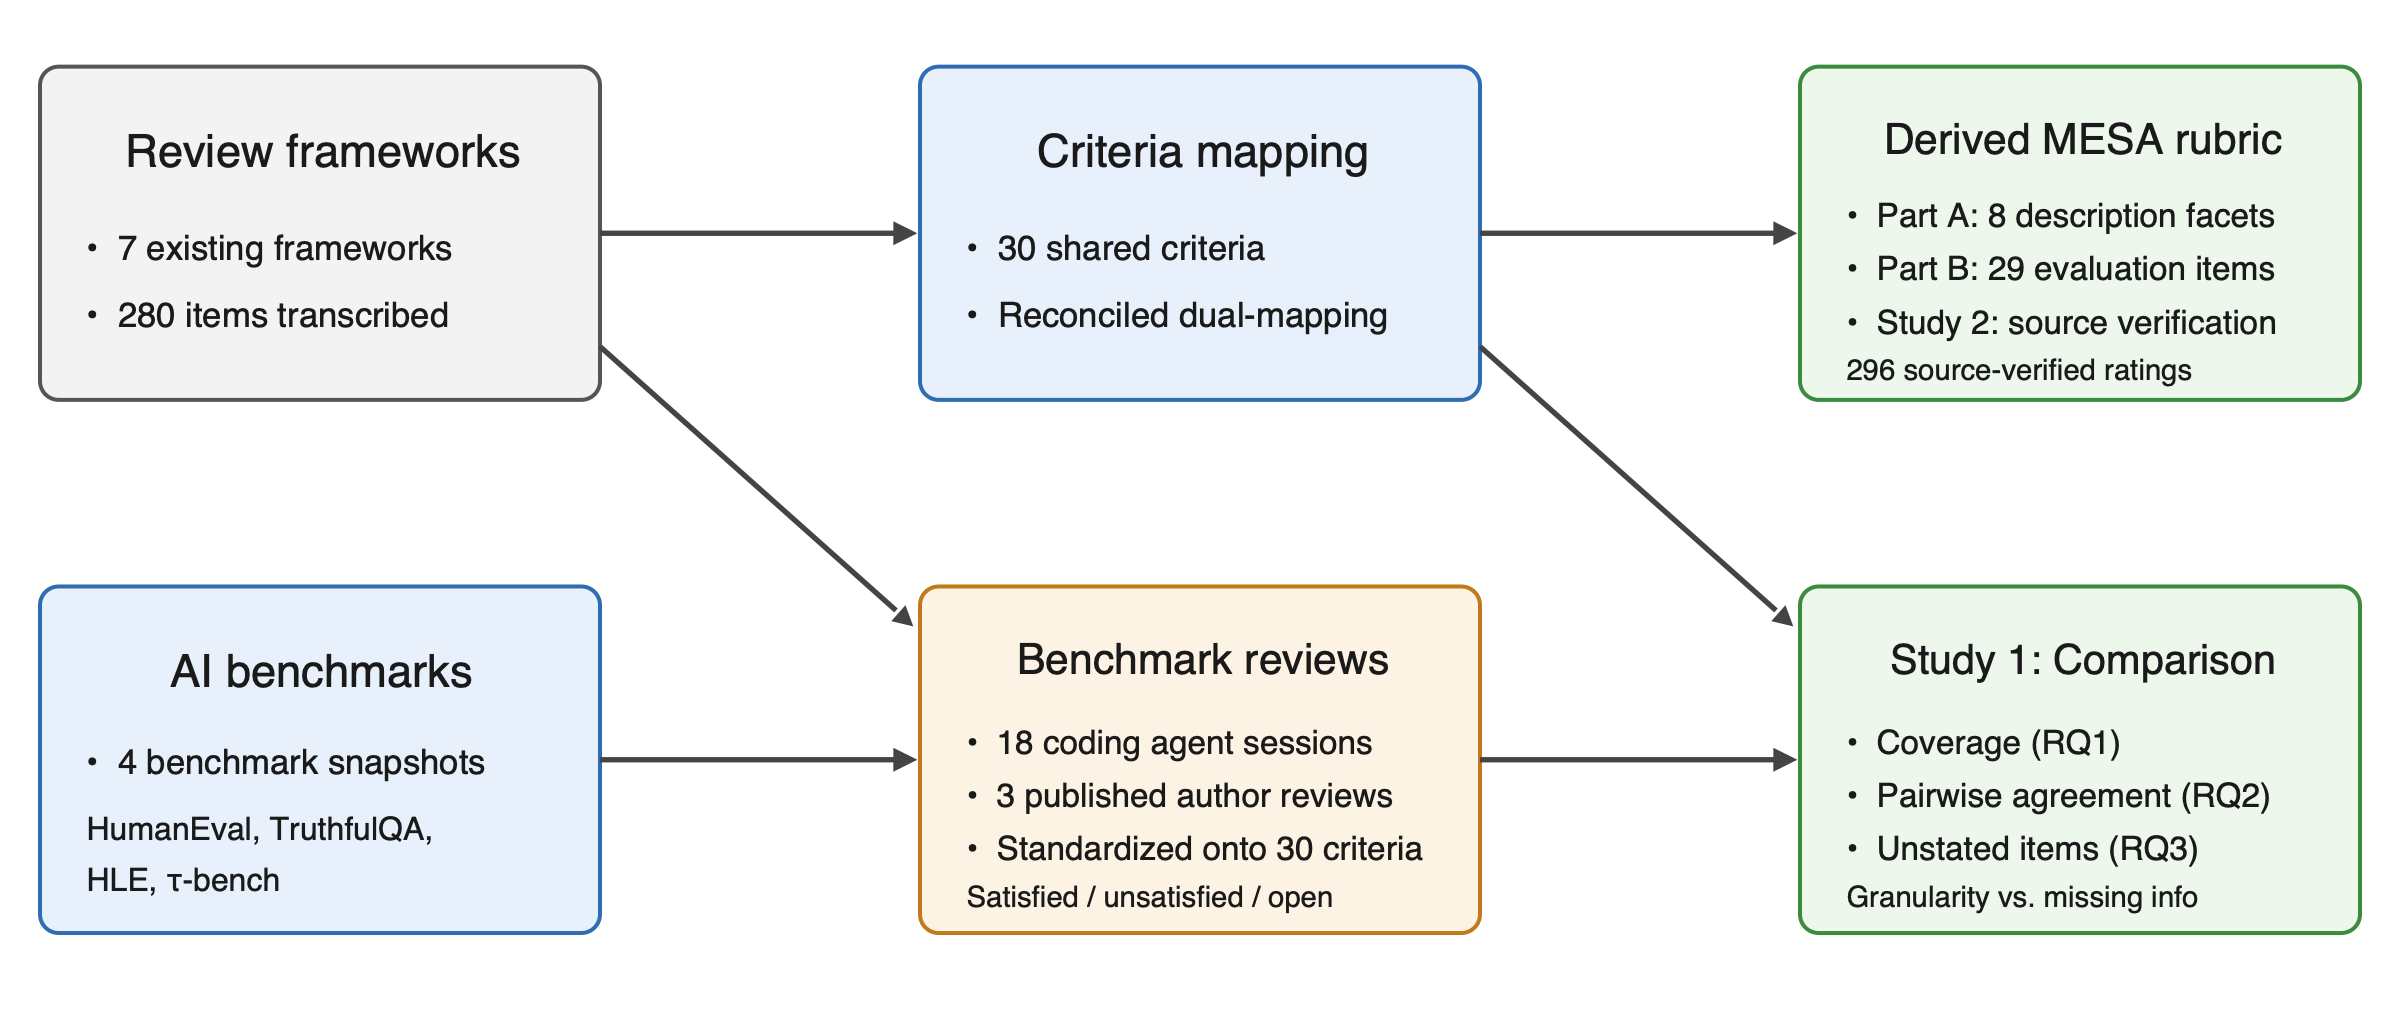
\includegraphics[width=0.92\textwidth]{figures/v4_study1_diagram.png}
\caption{Study 1: frameworks, mapping, agent sessions and the three comparisons (coverage, agreement, treatment of undocumented items).}
\label{fig:study1}
\end{figure*}

\begin{figure}[t]
\centering
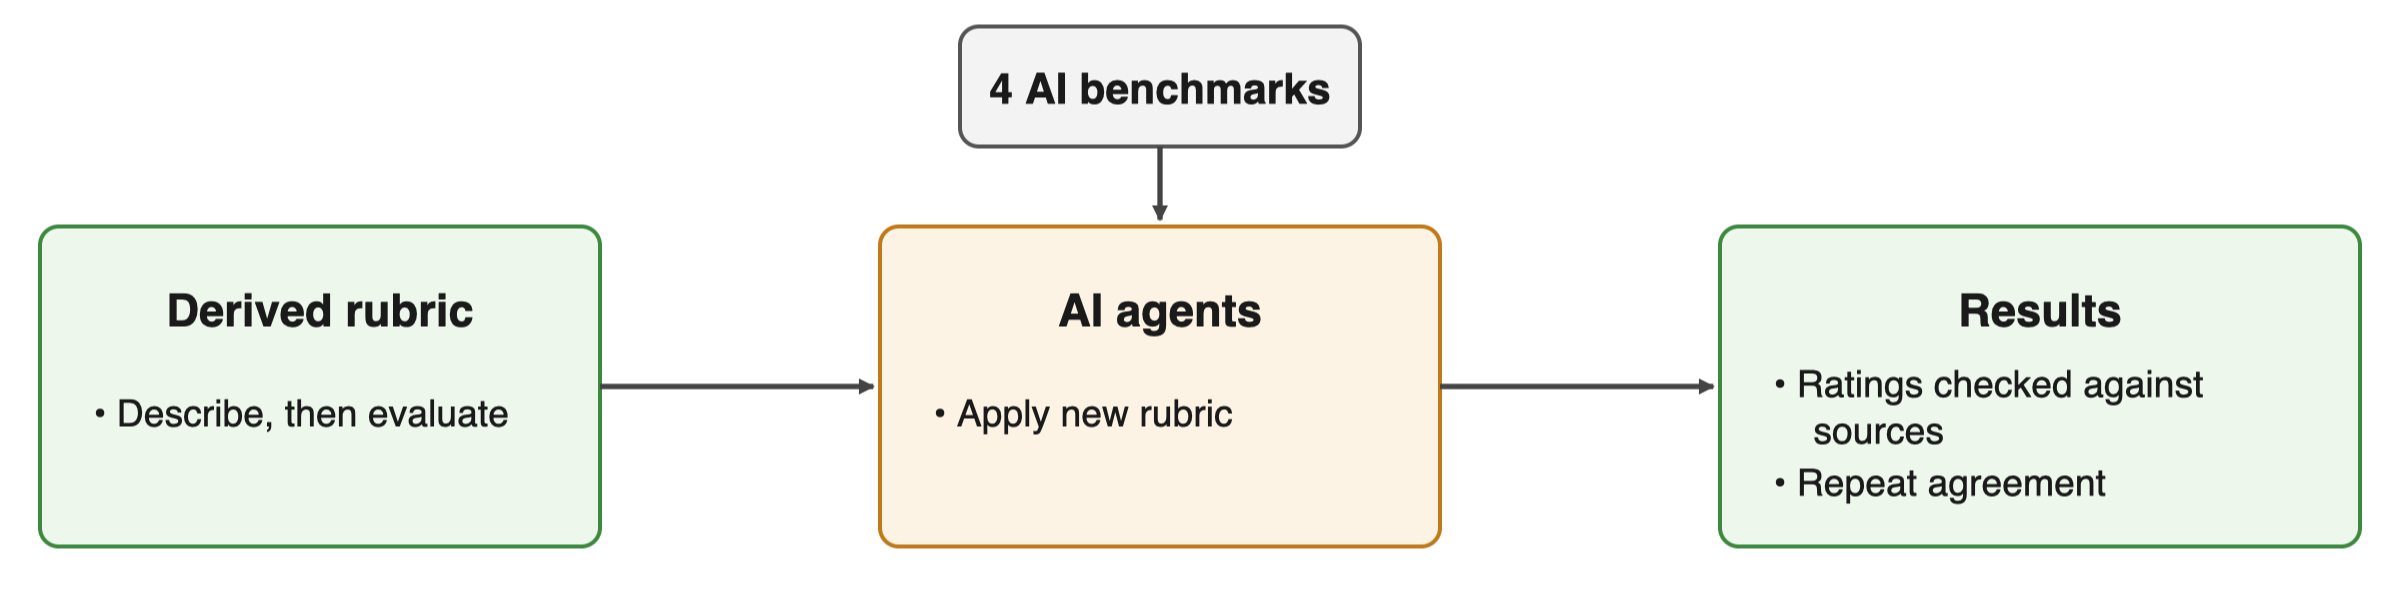
\includegraphics[width=\columnwidth]{figures/v4_study2_diagram.png}
\caption{Study 2: the MESA rubric applied twice per benchmark, with a source check of every rating against the sources it cites and a comparison of the repetitions.}
\label{fig:study2}
\end{figure}

\subsection{Benchmarks and frozen snapshots}
We evaluate four benchmarks that span code generation, truthfulness in question answering, frontier academic reasoning and multi-turn tool use, plus one tiny fictional benchmark used only for harness pilots before the study inputs were frozen. Table~\ref{tab:benchmarks} summarizes each snapshot's domain, published reviews, paper length, repository file count and prompt token range across sessions.

\begin{table*}[t]
\caption{Benchmark snapshots and the fictional pilot fixture evaluated in the study.}
\label{tab:benchmarks}
\centering
\small
\begin{tabularx}{\textwidth}{@{}llrrX@{}}
\toprule
\textbf{Benchmark} & \textbf{Earlier published reviews} & \textbf{Paper pages} & \textbf{Repository files} & \textbf{Estimated prompt size across sessions} \\
\midrule
HumanEval \cite{human_eval_repository} & BetterBench (47 items), How2Bench (aggregate) & 35 & 12 & 41,349--44,164 tokens \\
TruthfulQA \cite{truthfulqa_repository} & BetterBench (47 items) & 39 & 25 & 37,176--39,992 tokens \\
Humanity's Last Exam \cite{phan_etal_hle_2025} & None & 29 & 16 & 28,925--31,740 tokens \\
$\tau$-bench \cite{tau_bench_repository} & Agentic Benchmark Checklist (31 of 44 items) & 50 & 113 & 36,056--38,872 tokens \\
Pilot fixture (AddTwo) & None (pilots only) & 1 & 2 & 1,522--4,337 tokens \\
\bottomrule
\end{tabularx}
\end{table*}

Three benchmarks were chosen because the authors of at least one review framework had published an assessment of them:
\begin{itemize}
\item \textbf{HumanEval} \cite{human_eval_repository} is OpenAI's 164-problem Python code generation benchmark, reviewed item by item in the BetterBench database and included in How2Bench's aggregate survey. Its repository snapshot contains 12 files, including the execution module where candidate solutions run via an unrestricted execution call inside a reliability guard.
\item \textbf{TruthfulQA} \cite{truthfulqa_repository} is an 817-question benchmark testing whether language models repeat human falsehoods, reviewed item by item in the BetterBench database. Its repository snapshot contains 25 files (including evaluation datasets and earlier release files) and the scoring module, which at three sites appends a fixed no comment answer to the list of true reference answers when it is absent, before similarity scoring.
\item \textbf{$\tau$-bench} \cite{tau_bench_repository} evaluates tool-using agents interacting with simulated airline and retail users and databases under policy rules, reviewed by ABC authors on 31 of their 44 items. Its repository snapshot contains 113 files (largely saved historical trajectory logs alongside the environment, tool and task definitions).
\end{itemize}

The fourth benchmark, \textbf{Humanity's Last Exam (HLE)} \cite{phan_etal_hle_2025}, has no published review under any framework. It was added by the author's decision before the freeze as a prominent recent benchmark whose repository (16 files including judge scripts, rolling change logs and blocklists) is distributed separately from its gated 2,500-question dataset. The author obtained the dataset under its access terms and placed the text of the question items (with image bytes and author names omitted) and the dataset documentation inside the local snapshot alongside the repository files.

A fifth candidate, HELM \cite{liang_helm_2022}, was fetched and removed before the freeze because its 162-page paper produced prompts of about 167,000 tokens and its existing reviews were made from the paper alone. We treat all published reviews as reference points rather than gold standards: each is one team applying its own instrument on an unrecorded date, usually from the paper alone.

\subsection{Frameworks and where each applies}
The four general-purpose frameworks (BetterBench, ECBD, the Scorecard and the OECD facets) are applied to all four benchmarks (16 sessions). The two domain-specific frameworks are applied where their scope matches the benchmark: How2Bench on HumanEval (1 session) and ABC on $\tau$-bench (1 session), making 18 main framework sessions in Study 1. Because every item of Caliper presupposes a named target deployment culture or region and its only benchmark with an expert regional score was HELM (Southeast Asia), Caliper is included in the RQ1 mapping and coverage analysis but is not run in agent sessions. In Study 2, the MESA rubric is applied twice to each of the four benchmarks (8 main sessions), yielding 26 main sessions in total. After those sessions and their analysis, a recorded amendment added a second repetition of BetterBench and the Scorecard on HumanEval (2 sessions, same model, same frozen prompts, schemas and snapshot) to estimate same-framework repeat variation; those two sessions enter only the repeat-agreement counts of Section~\ref{sec:rq2}.

\subsection{Reviewers and session isolation}
\label{sec:reviewers}
All sessions use a single coding agent configuration: Claude Sonnet 5.5 invoked through the Claude Code command-line interface at medium effort \cite{anthropic_claude_code_cli}. Each session runs in a fresh empty temporary directory with standard input carrying the prompt, the default system prompt replaced by the study system instruction, user and project settings disabled, skills and built-in tools disabled, permission prompts denied, and the context compaction threshold set to its maximum so the supplied benchmark documents are never summarized away. The only tools exposed to the agent are two read-only Model Context Protocol (MCP) tools served over the benchmark's frozen repository snapshot: one to list available files and one to read numbered lines from a requested file (200 lines by default, while rejecting symbolic links, binary files and any path that resolves outside the snapshot root). The agent cannot run code, access the network, write files or read sibling directories.

Every prompt contains the study system instruction, one complete framework packet with verbatim item text and the framework's own scoring and guidance for undocumented items, a worked teaching example on a tiny fictional benchmark so the expected level of citation detail is clear, the benchmark documents (the text extracted from the paper, the top-level repository documentation, and for HLE the dataset documentation), and instructions to inspect the repository through the file reader before emitting a single structured response validated against the framework's schema. No per-session token, output, tool-call or wall-clock ceilings are imposed.

\textbf{Execution.} All 35 attempts (7 pilots, 26 main sessions and the 2 amendment sessions) ran on the same day, each completed on its first attempt, and no retry was needed, so the attempt cap of 36 was not exceeded. Every main response passed schema and structural validation, and the event log of every session reports Claude Sonnet 5.5 as the serving model. The 26 main sessions took 21 minutes in all, between 22 and 92 seconds each (median 51 seconds), and consumed 3,874,097 input tokens (uncached, cache-creation and cache-read input summed) and 199,133 output tokens; the two amendment sessions added 102 seconds, 410,952 input and 16,601 output tokens. In the 26 main sessions the agent made 50 file-reader calls in all, every one of which succeeded; 19 sessions made at least one call and 13 read at least one repository file (all 7 HumanEval sessions but the ECBD one, 5 of 6 HLE sessions, 1 of 6 TruthfulQA sessions and 1 of 7 $\tau$-bench sessions). No session used any tool other than the two repository reader tools. One harness defect appeared after the pilots and before the first main session: the initial freeze manifest recorded relative paths from the repository root while the runner resolved listed paths from the study directory, so the freeze check stopped the first main launch before any model call; the path resolution was corrected, the change recorded in the protocol, and the freeze manifest regenerated. No prompt, material, schema or analysis logic changed.

\subsection{Pre-experiment checks and pilots}
The study protocol requires ten checks before any main session, each with a pass condition: materials and reuse terms transcribed; every item classified as answerable or not from the inputs (238 yes, 25 with a declared target context, 11 partly, 6 no); mapping, recoding rules and published reviews finished; snapshots fetched and hashed; input sizes measured; one response schema per framework validated; an offline dry run of the whole analysis on synthetic responses; nine harness tests; seven pilots on the fictional two-task AddTwo fixture, one per prompt; and a cryptographic hash manifest of all 254 input files. All ten passed on the day of the sessions, in that order; the pilots completed on their first attempt in 21 to 45 seconds, passed validation, used only the two file-reader tools and returned the requested model, and no harness change followed them. Pilot judgments are never analyzed.

\subsection{Pre-registered hypotheses and analysis plan}
Five hypotheses were registered in the study protocol before the sessions. The protocol states them in plain words; the criterion and question identifiers below were attached when the analysis was written, before any session output was read, so that each could be counted:
\begin{itemize}
\item \textbf{H1:} Existing frameworks agree on documentation presence and licensing (C18, C19) and diverge on validity criteria (C01--C16).
\item \textbf{H2:} Much of the disagreement across frameworks on validity criteria comes from how each framework treats information the benchmark does not report (\emph{undocumented}), rather than from reading the benchmark sources differently.
\item \textbf{H3:} Several criteria appear in only one framework: maintenance and contact in BetterBench (C22), result presentation in How2Bench (C26), and descriptive instrument classification in the OECD facets (C30).
\item \textbf{H4:} Under the MESA rubric, items a benchmark does not report are recorded as \emph{Undocumented} (\emph{open}) where BetterBench and How2Bench record a low score or failure (\emph{not met} with \emph{undocumented}).
\item \textbf{H5:} The MESA rubric questions corresponding to the OECD facets with low 2023 rater agreement (B01/B16 for Capability, B04 for Coverage, and B13 for Specificity) are the questions whose ratings a human reviewer can least often confirm from the cited sources.
\end{itemize}

The analysis records keep their original field names: basis with evidence\_found, absence\_of\_information and defect\_found for the evidence; outcome with favorable, unfavorable and unresolved for the verdict; partial and unresolved\_by\_rule for the qualifiers; stated, shown, checked and insufficient\_evidence for the claimed, documented, verified and undocumented levels; and supported, weaker and not\_supported for the source check findings. All post-session analysis is performed deterministically offline without model calls or manual output repair. For every attempt, the analysis first validates the response against its schema, parses tool calls and token usage from the session event log, and checks every citation against the snapshot (verifying whether the source document exists, whether the quote matches exactly or after whitespace normalization, and whether the locator contains a line or page number). It then recodes item answers into verdicts and qualifiers, aggregates them to the 30 criteria, computes pairwise agreement across frameworks (both three-verdict agreement and strict agreement requiring the \emph{in part} qualifier to match), compares the agent's BetterBench verdicts with the BetterBench authors' published reviews on HumanEval and TruthfulQA, counts RQ3 conflicts per benchmark where one framework is \emph{not met} (\emph{undocumented}) and another is \emph{open} on the same criterion, and prepares every rubric rating with its cited sources for the source check. The five causes used to code the disagreements in Section~\ref{sec:rq2} were fixed when the analysis was written, before the sessions, and are not part of the frozen protocol. Because answers and ratings nested within benchmarks and frameworks are not independent random samples, we report exact counts and denominators rather than probability values, and we never compute a composite benchmark score.

\section{Results}
We report the pre-experiment results for RQ1 (Section~\ref{sec:rq1}) and the first half of RQ3 (Section~\ref{sec:rq3}), then the session results for RQ2, the second half of RQ3, and RQ4. All session counts are descriptive: answers and ratings are nested within benchmarks and frameworks, one agent configuration produced them, and agreement between frameworks does not make either of them right.

\subsection{RQ1: Coverage of shared criteria}
\label{sec:rq1}
Table~\ref{tab:coverage} presents the complete coverage matrix mapping the 280 items of the seven frameworks onto the 30 shared criteria. Across all 280 items, 180 items map to a single criterion, 94 items map to two criteria, and 6 items map to three criteria (SC-26 on design rationale and real world prediction, ABC-T.1 on tool versions, ABC-O.f.3 on preventing flaky tests, ABC-R.4 on updating tasks against overfitting, and the OECD Reproducibility and Variation facets), producing 386 item-to-criterion links in all.

\begin{table*}[t]
\caption{Items per shared criterion and framework.}
\label{tab:coverage}
\centering
\small
\begin{tabular}{@{}llrrrrrrrr@{}}
\toprule
\textbf{Id} & \textbf{Criterion} & \textbf{BetterBench} & \textbf{ECBD} & \textbf{Scorecard} & \textbf{How2Bench} & \textbf{ABC} & \textbf{Caliper} & \textbf{OECD} & \textbf{Frameworks} \\
\midrule
C01 & The ability under test is stated and made concrete & 2 & 2 & 3 & 2 & 1 &  & 1 & 6 \\
C02 & The intended use, users and real-world relevance are stated & 2 & 3 & 1 & 1 & 1 &  & 2 & 6 \\
C03 & Task selection is justified for the claimed ability & 4 & 3 & 5 & 2 & 1 &  &  & 5 \\
\midrule
C04 & The task set covers the ability and is representative & 2 & 5 & 4 & 5 &  & 5 & 1 & 6 \\
C05 & Tasks and reference answers were checked & 1 &  & 10 & 7 & 12 & 3 &  & 5 \\
\midrule
C06 & The scoring rule is described & 3 & 2 & 4 & 4 & 3 &  & 1 & 6 \\
C07 & The scoring implementation was checked and cannot be gamed & 1 & 1 & 8 & 1 & 18 &  &  & 5 \\
C08 & Aggregation and subscores are justified &  & 3 & 3 & 1 &  & 1 & 1 & 5 \\
C09 & Comparison points are justified & 3 &  & 3 &  & 2 &  & 1 & 4 \\
\midrule
C10 & Variation on repeated testing is reported &  &  & 2 & 3 & 1 &  & 2 & 4 \\
C11 & Prompting and setup are described and their effect tested & 2 & 3 & 3 & 6 &  &  &  & 4 \\
C12 & Uncertainty and statistical support are reported & 1 & 2 & 3 & 1 & 2 &  &  & 5 \\
C13 & Shortcuts, confounds and chance were investigated &  & 1 & 12 & 1 & 6 & 2 & 1 & 6 \\
\midrule
C14 & Exposure of test material in training data was assessed & 2 &  & 1 & 1 & 2 &  &  & 4 \\
C15 & Rules for training on the test and for repeated submission are stated & 1 &  &  &  & 1 &  &  & 2 \\
C16 & Claims about performance beyond the test are supported & 1 & 1 & 6 & 1 &  & 1 & 2 & 6 \\
C17 & Fairness across systems and conditions is addressed &  & 1 & 1 &  &  & 1 & 2 & 4 \\
\midrule
C18 & Materials and instructions for repeating the evaluation are provided & 10 &  & 3 & 11 & 3 &  & 1 & 5 \\
C19 & Terms of access and license are stated & 1 &  &  & 2 &  &  &  & 2 \\
C20 & Versions and changes are recorded & 3 &  & 1 &  & 3 &  & 2 & 4 \\
C21 & Limitations and flaws are stated and claims stay within the evidence & 4 &  & 6 &  & 4 &  &  & 3 \\
C22 & Maintenance and a contact exist & 4 &  &  &  &  &  &  & 1 \\
\midrule
C23 & Transfer to another cultural or deployment context is assessed &  &  &  &  &  & 28 & 1 & 2 \\
C24 & Harmful or sensitive content is handled & 1 &  &  & 3 &  & 1 &  & 3 \\
C25 & The systems evaluated and the difficulty of the benchmark are examined &  &  &  & 6 &  &  & 1 & 2 \\
C26 & Results are presented and explained &  &  &  & 6 &  &  &  & 1 \\
C27 & Data provenance and collection are documented & 7 & 1 & 4 & 5 &  & 1 & 2 & 6 \\
C28 & The evaluation environment is controlled and isolated from answers &  &  & 3 &  & 7 &  & 1 & 3 \\
C29 & Domain experts or users took part in design or review & 1 & 1 & 2 &  &  & 2 &  & 4 \\
\midrule
C30 & What kind of instrument the benchmark is, recorded as a description &  &  &  &  &  &  & 10 & 1 \\
\midrule
\multicolumn{2}{@{}l}{Total items in framework} & 47 & 20 & 68 & 55 & 44 & 28 & 18 & 280 \\
\multicolumn{2}{@{}l}{Total item-to-criterion links} & 56 & 29 & 88 & 69 & 67 & 45 & 32 & 386 \\
\multicolumn{2}{@{}l}{Criteria covered (out of 30)} & 21 & 14 & 22 & 20 & 16 & 10 & 17 & --- \\
\bottomrule
\end{tabular}
\par\vspace{2pt}\raggedright\footnotesize An empty cell means the framework has no item for the criterion. Counts follow the finalized mapping after reconciling the author's independent mapping with the assistant model's draft.
\end{table*}

Four structural findings stand out in Table~\ref{tab:coverage}:
\begin{enumerate}
\item \textbf{No criterion is universal, and coverage breadth varies from 10 to 22 criteria per framework.} No row of Table~\ref{tab:coverage} is covered by all seven frameworks, primarily because Caliper specializes in regional transfer (covering 10 of 30 criteria) and ECBD focuses on construct and evidence design without software release or contamination items (covering 14 of 30 criteria). Even the broadest frameworks, the Scorecard (22 criteria), BetterBench (21 criteria) and How2Bench (20 criteria), each omit at least eight criteria asked by their peers. Across the 30 criteria, 7 are covered by six frameworks (C01, C02, C04, C06, C13, C16, C27), 6 by five frameworks (C03, C05, C07, C08, C12, C18), 7 by four frameworks (C09, C10, C11, C14, C17, C20, C29), 3 by three frameworks (C21, C24, C28), 4 by two frameworks (C15, C19, C23, C25), and 3 by one framework only, confirming Hypothesis H3: maintenance and user contact in BetterBench (C22, 4 items), visual and explanatory presentation of experiment results in How2Bench (C26, 6 items), and descriptive instrument classification in the OECD facets (C30, 10 items).
\item \textbf{Item granularity is highly skewed across criteria.} Six criteria absorb 164 of the 386 item links (42.5\%): checking tasks and reference answers (C05, 33 links), checking that the scoring implementation cannot be gamed (C07, 29 links), regional transfer (C23, 29 links, 28 of them from Caliper), repeatability materials and instructions (C18, 28 links, 21 of them from BetterBench and How2Bench), investigating shortcuts, confounds and chance (C13, 23 links, 12 from the Scorecard and 6 from ABC), and task coverage and representativeness (C04, 22 links). At the other extreme, rules for training on the test and repeated submission (C15, 2 links: BB-25 and ABC-R.4) and access and licensing terms (C19, 3 links: BB-37, H2B-46 and H2B-49) receive minimal item counts.
\item \textbf{Within a single criterion, frameworks allocate very different numbers of items.} On C07 (whether the scoring implementation was checked and resists gaming), BetterBench, ECBD and How2Bench ask 1 item each, the Scorecard asks 8 items, and ABC asks 18 items across unit tests, fuzz tests, end-to-end tests, state matchers and LLM judges. Similarly, on C05 (checking tasks and reference answers), BetterBench has 1 item (BB-42 on annotation documentation), whereas the Scorecard has 10 items and ABC has 12 items. Because any single not met item makes a criterion verdict not met under our aggregation rule, a framework asking 12 or 18 detailed questions about grading and task verification has a much higher structural bar for a met criterion verdict than a framework asking one general question.
\item \textbf{Independent mapping comparison exposed 100 item-level differences before freeze.} Comparing the assistant model's initial mapping draft with the author's independent mapping across all 280 items showed identical criterion sets on 180 items (of which 178 stayed unchanged and 2 received a second criterion during reconciliation for section consistency) and differing criterion sets on 100 items. Most differences turned on whether an item touches a secondary criterion alongside its primary criterion: on 56 items the finalized mapping kept the assistant model's draft, on 28 it adopted the author's independent reading, on 4 it took the union of both readings, and on 12 it selected a third reading that reconciled the two.
\end{enumerate}

\subsection{RQ2: Agreement across frameworks}
\label{sec:rq2}
Table~\ref{tab:grid-humaneval} gives the recoded verdict of every applied framework on every criterion it covers for HumanEval, with the MESA rubric's first repetition in the last column for reference only (it enters no Study 1 count); the counts below cover all four benchmarks. The 18 framework sessions produced 711 item answers, of which 52 OECD descriptive facet answers are not recoded. Three patterns are visible before any count. First, the Scorecard is not met on most of the criteria it covers on every benchmark, and most of those cells carry the $r$ qualifier (every one on HumanEval, 8 of 15 on HLE): 123 of its 272 item answers rest on undocumented evidence, and its rule turns each of them into \emph{unsatisfied}. Second, ECBD is never not met: with no scale of its own it records evidence or its absence, so it is met where the others are met and open where the others are not met under the framework's rule. Third, BetterBench sits between the two, met in part on many validity criteria and not met under the framework's rule on the contamination, materials, versioning and maintenance criteria (C14, C18, C20, C22) on every benchmark and on submission rules (C15) on three of the four.

\begin{table}[t]
\caption{Verdicts per criterion on HumanEval.}
\label{tab:grid-humaneval}
\centering
\small\begin{tabular}{lcccccc}\toprule
\textbf{Criterion} & \textbf{BetterBench} & \textbf{ECBD} & \textbf{Scorecard} & \textbf{How2Bench} & \textbf{OECD facets} & \textbf{Rubric} \\
\midrule
C01 & (+) & (+) & + & + & d & (+) \\
C02 & -r & (+) & ? & + & d & (+) \\
C03 & (+) & (+) & -r & + &  & (+) \\
C04 & -r & (+) & -r & -r & - & (+) \\
C05 & ? &  & -r & -r &  & ? \\
C06 & -r & + & -r & -r & d & (+) \\
C07 & (+) & + & -r & -r &  & (+) \\
C08 &  & (+) & -r & -r & d & (+) \\
C09 & -r &  & -r &  & d & (+) \\
C10 &  &  & -r & -r & - & (+) \\
C11 & (+) & (+) & -r & -r &  & + \\
C12 & (+) & (+) & -r & ? &  & ? \\
C13 &  & + & -r & -r & - & (+) \\
C14 & -r &  & -r & + &  & (+) \\
C15 & -r &  &  &  &  & ? \\
C16 & (+) & + & -r & + & d & (+) \\
C17 &  & ? & ? &  & - & (+) \\
C18 & -r &  & -r & -r & - & (+) \\
C19 & + &  &  & + &  & (+) \\
C20 & -r &  & ? &  & - & ? \\
C21 & -r &  & -r &  &  & (+) \\
C22 & -r &  &  &  &  & (+) \\
C23 &  &  &  &  & - & ? \\
C24 & -r &  &  & -r &  & (+) \\
C25 &  &  &  & -r & d & (+) \\
C26 &  &  &  & -r &  & + \\
C27 & -r & + & ? & -r & d & (+) \\
C28 &  &  & -r &  & d & (+) \\
C29 & -r & ? & -r &  &  & ? \\
C30 &  &  &  &  & d &  \\
\bottomrule\end{tabular}
\par\vspace{2pt}\raggedright\footnotesize Repetition 1. +: met; (+): met in part; -: not met; ?: open; d: descriptive only; r: not met by the framework's rule for undocumented items. The last column is the MESA rubric, repetition 1, for reference only.
\end{table}

\begin{table}[t]
\caption{Agreement between framework pairs per benchmark.}
\label{tab:pairwise}
\centering
\small\begin{tabular}{lrrrr}\toprule
\textbf{Pair} & \textbf{HumanEval} & \textbf{TruthfulQA} & \textbf{HLE} & \textbf{$\tau$-bench} \\
\midrule
BetterBench and ECBD & 6/11 (4) & 9/11 (7) & 7/11 (6) & 7/11 (3) \\
BetterBench and Scorecard & 8/17 (7) & 10/17 (7) & 7/17 (6) & 10/17 (8) \\
BetterBench and OECD facets & 3/3 (3) & 0/3 (0) & 2/3 (2) & 2/3 (2) \\
BetterBench and How2Bench & 9/15 (6) &  &  &  \\
\midrule
ECBD and Scorecard & 2/14 (1) & 6/14 (3) & 4/14 (3) & 3/14 (2) \\
ECBD and OECD facets & 0/3 (0) & 0/3 (0) & 0/3 (0) & 0/3 (0) \\
ECBD and How2Bench & 4/12 (1) &  &  &  \\
OECD facets and Scorecard & 4/6 (4) & 4/6 (4) & 5/6 (5) & 4/6 (4) \\
\midrule
How2Bench and Scorecard & 10/16 (10) &  &  &  \\
How2Bench and OECD facets & 4/4 (4) &  &  &  \\
\midrule
ABC and BetterBench &  &  &  & 10/13 (7) \\
ABC and ECBD &  &  &  & 3/7 (1) \\
ABC and Scorecard &  &  &  & 13/15 (12) \\
ABC and OECD facets &  &  &  & 3/4 (3) \\
\midrule
All pairs & 50/101 (40) & 29/54 (21) & 25/54 (22) & 55/93 (42) \\
\bottomrule\end{tabular}
\par\vspace{2pt}\raggedright\footnotesize Repetition 1. Criteria with the same verdict over criteria both frameworks cover; in parentheses, matches that also agree on the \emph{in part} qualifier. An empty cell is a pair not applied to that benchmark.
\end{table}

Table~\ref{tab:pairwise} gives the pairwise counts. Over the 32 framework pairs and 302 criterion comparisons, 159 (53\%) have the same verdict and 125 (41\%) also match on the \emph{in part} qualifier. That figure is a property of the translation as much as of the frameworks: it depends on how the items were mapped to criteria and on the aggregation rule, which is why the majority-rule count is reported beside it. Agreement is highest where both frameworks are audit-style checklists with the same rule for undocumented items: ABC and the Scorecard agree on 13 of 15 shared criteria on $\tau$-bench, and How2Bench and the Scorecard on 10 of 16 on HumanEval. It is lowest between ECBD and the Scorecard (2 to 6 of 14 on each benchmark) and between ECBD and the OECD evaluative facets (0 of 3 on every benchmark), that is, between the frameworks whose treatment of undocumented items differs most. The OECD evaluative facets, which classify a property rather than record documentation, account for 14 of the 32 pairs and 56 of the 302 comparisons with 31 agreements; without them the 18 remaining pairs agree on 128 of 246. Under a majority rule in place of the any-not met aggregation (ties to not met), the 302 comparisons agree on 148 instead of 159, so the aggregation rule moves the total by little. The amendment gives a first estimate of how much of this is run-to-run variation of the agent rather than a difference between instruments. On HumanEval the second BetterBench run reaches the same criterion verdict as the first on 19 of 21 criteria (18 with the \emph{in part} qualifier) and the same item score on 40 of 47 items; the second Scorecard run matches the first on 20 of 22 criteria and 56 of 68 items. Both same-framework counts are well above the 8 of 17 that BetterBench and the Scorecard share on the same benchmark. All four criterion level changes between repetitions involve the \emph{undocumented} qualifier (BetterBench C12 and C24 moved between met in part and not met under the framework's rule; the Scorecard's C02 and C20 moved from open to not met under the framework's rule), and 7 of the 12 Scorecard item changes are \emph{not applicable} in one run and \emph{unsatisfied} in the other. Hypothesis H1 holds in direction: on the two documentation criteria (C18 materials and C19 license) 17 of 19 pair comparisons agree, on the sixteen validity criteria (C01 to C16) 117 of 221 agree, and on the remaining criteria 25 of 62.

\textbf{Disagreements and their causes.} Of the 143 criterion level disagreements, 97 have a not met verdict qualified as \emph{undocumented} on at least one side: 85 oppose a met verdict to a not met one that follows from a rule for undocumented items, 12 oppose such a not met verdict to an open one, and the remaining 46 oppose met to not met without the qualifier (29), met to open (11) or not met to open (6). Every disagreement was coded with one of the five causes fixed in the analysis plan before the sessions; the coding was done by the assistant model from the saved reasons, cited sources and the snapshot, with the evidence for each code recorded, and the author's review of it is pending. A disagreement was coded to the rule for undocumented items when both sides recorded the same absence and only its scoring differed, to item granularity when the deciding item had no counterpart in the other framework, to reading when the two frameworks' items ask about different things under the same criterion, to threshold when both cite the same passage and grade it differently, and to sources read when one side cites material the other did not open. The counts are: a single narrow item driving the criterion verdict under the any-not met aggregation rule (\emph{item granularity}) 50; a different rule for the same undocumented item (\emph{rule for undocumented items}) 42; a different reading of the criterion, for instance a documentation item against an OECD classification of the property itself (\emph{reading}) 42; a different threshold for the same evidence 8; and different sources read 1. Among the 97 disagreements with an \emph{undocumented} qualified side, 42 are coded to the rule for undocumented items, 37 to granularity and 18 to reading. Read with care, these counts say that under this mapping and agent setup the disagreements are consistent with differences in framework design: the rule for undocumented items and item granularity together account for 92 of the 143. The single case coded to sources read (ABC citing the dependency installation configuration on $\tau$-bench where the Scorecard read only the paper) does not show that reviewers rarely interpret evidence differently; a different interpretation of the same passage would appear under reading or threshold, which together hold 50 of the 143. H2 is therefore supported only in part, and only to the extent that the coding holds up under the author's review.

\textbf{A worked example.} Criterion C12, uncertainty and statistical support, on HumanEval shows what a disagreement looks like once it is traced back to the items. BetterBench asks one item, BB-22, on statistical significance or uncertainty quantification; the agent scored it 10 because the paper justifies an unbiased pass@k estimator with 200 samples but gives no confidence intervals, so the evidence is documented and the verdict is met in part. The Scorecard asks three items: SC-13 on an appropriate estimator is satisfied on the same passage, while SC-14 on a power justification and SC-15 on confidence intervals are unsatisfied because the paper reports neither, so under the any-not-met rule the criterion is not met with the \emph{undocumented} qualifier. ECBD's Q14 records that no validity evidence supports the item set and Q20 credits the proof that the estimator is unbiased, which gives met in part. How2Bench's H2B-09 asks about the sampling of data, which the agent judged not to apply, so its verdict is open. All four readings cite the same places in the paper, Section 2.1, Table 1 and Appendix A, and none of them disputes a fact about HumanEval. What differs is what each framework requires before it is satisfied, intervals and power for the Scorecard, any treatment of uncertainty for BetterBench, a sampling description for How2Bench, and how many items each spends on the criterion. Two of the pairs are coded to the rule for undocumented items and three to a different reading of the criterion, and the example shows that the two categories can shade into each other: a narrow item fails for want of a number while a broader item passes on the same passage.

\textbf{Agent versus the BetterBench authors.} On the 21 criteria BetterBench covers, the agent's BetterBench application reaches the same verdict as the authors' published review on 15 criteria for HumanEval (11 when the \emph{in part} qualifier must also match) and on 17 for TruthfulQA (13 strict). On HumanEval the agent is not met under the framework's rule where the authors were met on four criteria (C02 intended use, C04 coverage, C06 scoring rule and C29 expert involvement) and met in part where the authors were not met under the framework's rule on two (C11 prompting and C12 uncertainty). On TruthfulQA all four differences run one way: the authors were not met under the framework's rule and the agent met on C02, C03 task justification, C04 and C24 harmful content, and because the authors' review carries no date we cannot tell whether those differences reflect the 2025 repository changes or reviewer differences. Both applications are not met only under the framework's rule, never for contradicted evidence: 13 of 13 not met agent criteria on HumanEval and 7 of 7 on TruthfulQA carry the qualifier, as do 11 of 11 in each published review.

\textbf{Repository inspection.} Six of the seven HumanEval sessions read the execution module; the ECBD session made no file-reader call. Of the six, one (the MESA rubric, repetition 2) recorded the contradiction the protocol asked about, rating B28 \emph{Contradicted} because the repository documentation says the execution call is deliberately commented out while the direct execution call is active in the implementation and the guard states that it is not a sandbox. The Scorecard session noted on SC-64 that the guard is explicitly not a security boundary, and the first rubric repetition repeated the repository documentation's claim that execution is commented out by default on B18 without checking it against the implementation. No TruthfulQA session opened the scoring module; the only TruthfulQA session that read any repository file (BetterBench) read the main evaluation script, so the modification of reference answers before scoring in the scoring module (three sites that append a fixed answer to the reference list) went unnoticed in all six TruthfulQA sessions, and three of them (OECD, Scorecard and the first rubric repetition) made no file-reader call at all. The $\tau$-bench sessions read the least: only ABC session read repository files (two), although all seven received a 113-file snapshot.

\subsection{RQ3: Information a benchmark does not report}
\label{sec:rq3}
RQ3 asks how each framework treats information that a benchmark paper and repository do not report, and how much of the apparent negativity or disagreement in benchmark reviews is driven by those rules rather than by problems the sources show. We answer RQ3 in two parts: first from the frameworks' documented rules and the recoded published reviews (completed before any session), and second from the conflicts across frameworks observed in the live agent sessions.

Table~\ref{tab:missing-rules} compares the documented rules for undocumented items across all seven existing frameworks and the MESA rubric. The seven existing frameworks split into two incompatible camps:
\begin{itemize}
\item \textbf{Five frameworks penalize undocumented items by design.} BetterBench assigns 0 when an item is neither acknowledged nor addressed and 5 when it is mentioned without being addressed \cite{reuel_betterbench}. The Scorecard of AI Benchmark Quality allows vague or absent documentation to mark an item \emph{unsatisfied}, and if that item is a baseline item, the entire dimension becomes unscorable and the evaluation is classed as invalid \cite{san_joaquin_scorecard_2026}. How2Bench labels any step without explicit textual evidence in the paper as \emph{not mentioned} and groups \emph{not mentioned} with not done \cite{cao_how2bench_2025}. The ABC scores any undocumented item 0 without a separate category for undocumented items \cite{zhu_agentic_benchmark_checklist_2025}. Caliper returns \emph{Unknown} at the checklist item level when evidence is insufficient, but its 1 to 5 dimension rubrics score documented awareness of regional transfer, so an absent discussion in the benchmark documentation lowers the dimension score to 1 or 2 \cite{corona_benchmark_caliper_2026}.
\item \textbf{Two frameworks record undocumented items without a negative score.} ECBD records that a justification or validity support is not stated in the benchmark documentation without scoring it \cite{liu_ecbd_2024}. The OECD facets allow N/A on Reliability when the testing methodology or common use is unclear, while treating non-evaluative facets as neutral descriptions \cite{cohn_hernandez_orallo_oecd_2023}.
\end{itemize}

\begin{table*}[t]
\caption{Treatment of undocumented items by framework.}
\label{tab:missing-rules}
\centering
\small
\begin{tabularx}{\textwidth}{@{}llXl@{}}
\toprule
\textbf{Framework} & \textbf{Separate missing value?} & \textbf{Rule for undocumented items} & \textbf{Resulting verdict} \\
\midrule
BetterBench & No (n/a is for irrelevance only) & Criterion neither acknowledged nor addressed receives 0; mentioned but not provided receives 5 (Appendix F). & Not met (\emph{undocumented}) \\
ECBD & Yes (free-text note) & Describe, justify and support answers record what is stated; absence of justification or validity evidence is noted as absent, not scored. & Open \\
Scorecard & No (not applicable is for irrelevance) & Vague or absent documentation can make an item \emph{unsatisfied}; an unsatisfied baseline item makes the dimension unscorable (Appendix A.1). & Not met (\emph{undocumented}) \\
How2Bench & No & Benchmark is labeled \emph{not mentioned} unless the paper contains explicit textual evidence; \emph{not mentioned} is grouped with not done (Sections 4.2, 7.3). & Not met (\emph{undocumented}) \\
ABC & No & An item the benchmark does not document or report receives 0 with a short reason (Section 5.1, Appendix D). & Not met (\emph{undocumented}) \\
Caliper & At item level (\emph{Unknown}), not dimension level & Item scoring returns \emph{Unknown} when evidence is insufficient; dimension rubrics (1 to 5) score documented regional awareness, so an absent discussion lowers the score. & Item: Open; Dimension: Not met (\emph{undocumented}) \\
OECD facets & Only on Reliability (N/A) & Reliability allows N/A when methodology is unclear; other facets require choosing a listed value. & Reliability: Open; Descriptive: Not recoded \\
MESA rubric & Yes (\emph{Undocumented}) & Silence is recorded as \emph{Undocumented} with what was looked for noted; \emph{Contradicted} is reserved for cited defects. & Open \\
\bottomrule
\end{tabularx}
\end{table*}

To see what this split does to real benchmark reviews before any agent session runs, we recoded the three item-level reviews published by the framework authors themselves on our benchmarks: BetterBench's 47-item review of HumanEval, BetterBench's 47-item review of TruthfulQA, and ABC authors' 31-item review of $\tau$-bench. Table~\ref{tab:earlier-reviews} reports both the item-level and criterion level recodings after excluding the two unanswerable maintenance items (BB-45 and BB-46).

\begin{table*}[t]
\caption{Recoded verdicts of the published reviews.}
\label{tab:earlier-reviews}
\centering
\small
\begin{tabularx}{\textwidth}{@{}llrrrrrrX@{}}
\toprule
\textbf{Benchmark} & \textbf{Published review} & \textbf{Answerable items} & \textbf{Met} & \textbf{Met in part} & \textbf{Not met (undocumented)} & \textbf{Not met (contradicted)} & \textbf{Open (n/a)} & \textbf{Aggregated criterion verdicts across covered criteria} \\
\midrule
HumanEval & BetterBench (47 items; 2 unanswerable excluded) & 45 & 26 & 3 & 14 & 0 & 2 & 21 criteria: 9 Met (C01--C04, C06, C07, C16, C19, C29), 0 Met in part, 11 Not met (undocumented) (C09, C11, C12, C14, C15, C18, C20, C21, C22, C24, C27), 0 Not met (contradicted), 1 Open (C05) \\
\midrule
TruthfulQA & BetterBench (47 items; 2 unanswerable excluded) & 45 & 22 & 8 & 15 & 0 & 0 & 21 criteria: 7 Met (C01, C06, C07, C09, C12, C16, C19), 3 Met (\emph{in part}: C05, C11, C21), 11 Not met (undocumented) (C02--C04, C14, C15, C18, C20, C22, C24, C27, C29), 0 Not met (contradicted), 0 Open \\
\midrule
$\tau$-bench & Agentic Benchmark Checklist (31 of 44 items assessed) & 31 & 17 & 0 & 9 & 2 & 3 & 15 criteria: 5 Met (C01--C03, C05, C06), 2 Met (\emph{in part}: C18, C28), 6 Not met (undocumented) (C09, C12, C14, C15, C20, C21), 2 Not met from defect (C07, C13), 0 Open \\
\bottomrule
\end{tabularx}
\par\vspace{2pt}\raggedright\footnotesize Unanswerable items BB-45 and BB-46 excluded (the authors' 0 on BB-45 for TruthfulQA is the one unmarked not met BetterBench answer in the recoded file).
\end{table*}

The numbers in Table~\ref{tab:earlier-reviews} show why separating undocumented items from defects is central to benchmark evaluation:
\begin{itemize}
\item On \textbf{HumanEval}, the BetterBench authors gave 26 answerable items 15, 3 items 10, 2 items n/a, and 14 items 0 or 5. Each of those 14 records an absence: seven unperformed design or evaluation steps (no human baseline, input sensitivity study, canary string, contamination task, uncertainty interval, harmful content assessment or peer-reviewed venue) and seven absent repository or metadata artifacts (no API wrapper, replication script, build status badge, release requirements, persistent identifier beyond the paper, metadata file or documentation standard). Aggregated to the 21 criteria BetterBench covers, all 11 not met criterion verdicts carry the \emph{undocumented} qualifier and none rests on contradicted evidence about HumanEval's tasks or grading.
\item On \textbf{TruthfulQA}, the authors gave 22 answerable items 15, 8 items 10, and 15 items 0 or 5 (11 zeros for absent items and 4 fives where a topic was mentioned but not addressed). Again all 11 not met criterion verdicts carry the qualifier and none records contradicted evidence.
\item On \textbf{$\tau$-bench}, ABC authors scored 31 of their 44 items: 17 received 1 with evidence, 3 tool items received 1 because the benchmark uses no external tools (recoded as \emph{open} with \emph{not applicable}), and 11 received 0. Nine of the zeros state that the paper does not specify, discuss or report the item (\emph{undocumented}); only two (ABC-O.b.3 and ABC-O.g.3) identify a defect, that a subset of tasks has empty ground truth and allows guessing. At the criterion level 6 of the 8 not met criteria are not met under the framework's rule and 2 (C07 and C13) reflect the defect.
\end{itemize}

\textbf{Conflicts in the sessions.} The second part counts, per benchmark, the criteria where one framework records an absence as \emph{not met} (\emph{undocumented}) while another framework records the same absence on the same snapshot as \emph{open}. There are 9 such criteria: 6 on HumanEval (C02, C05, C12, C20, C27 and C29, with BetterBench, the Scorecard or How2Bench on the not met side and the Scorecard, ECBD, How2Bench or BetterBench on the open side), none on TruthfulQA, 2 on HLE (C02 and C07) and 1 on $\tau$-bench (C27). The count is small because the open verdict is rare among the applied frameworks: only ECBD leaves an absence open by design, and the Scorecard and BetterBench do so only through inapplicability. The larger effect of the rules shows in the 85 disagreements of Section~\ref{sec:rq2} where an absence scored not met by one framework faces a met verdict from another, and in the 210 of 711 Study 1 item answers (30\%) that carry the \emph{undocumented} qualifier, that is, that are not met because the framework's rule turns an absence or a bare acknowledgment into a failing score: 123 of 272 Scorecard answers, 52 of 188 BetterBench answers, 23 of 55 How2Bench answers and 12 of 44 ABC answers. Under a rule that keeps undocumented items apart, every one of those 210 answers would be open. The agent recorded contradicted evidence on only 13 of the 711 Study 1 answers: 9 Scorecard, 2 BetterBench and 2 ABC answers across the four benchmarks. Three different things can lie behind an undocumented answer. The item may be a reporting requirement, in which case the missing report is exactly the failure the framework set out to find, and the framework is entitled to score it not met. The item may ask about a practice, such as a contamination check, that the authors may have carried out without reporting it, in which case the sources leave the practice unknown. Or the sources may show that the practice was not done or was done wrongly, which the evidence value records as contradicted. The \emph{undocumented} qualifier pools the first two cases and this study does not separate them, so the comparison above is between answers whose evidence was undocumented and answers whose evidence was contradicted, not between failures of reporting and failures of practice. The qualifier records that a verdict rests on an absence; it does not say that the framework was wrong to score it.

\subsection{RQ4: The MESA rubric}
\label{sec:rq4}
The eight rubric sessions produced 64 description facet values and 232 Part B ratings. The source check reported below found 21 of the 232 ratings overstated and 19 of the 64 facet values overstated or not confirmed, so the results are read with those failures in view. Across the 232 ratings the levels were \emph{Documented} 123 times, \emph{Verified} 52, \emph{Undocumented} 20, \emph{Not applicable} 18, \emph{Claimed} 14 and \emph{Contradicted} 5. The five contradictions are the HumanEval repository documentation claim that execution is commented out against the active execution call in the code (B28, repetition 2), the HumanEval task count of 164 against 158 in the paper's appendix (B20, repetition 2), the HLE filtering of questions with the same models that are later evaluated under different sampling settings (B17, repetition 1), and the $\tau$-bench paper's own appendix checklist, which claims error bars that do not appear in its results (B12, both repetitions).

\textbf{Automated citation checks.} The Part B rubric ratings carry 271 citations, 1.2 per rating, against 0.9 per answer for BetterBench, 0.6 for the Scorecard and 1.8 for ECBD. For 260 the source string names a document in the snapshot as written; the 11 others name real repository files without the repository directory prefix, which the automated checker counts as unmatched. The quote matches the source exactly in 121 cases and after whitespace normalization in 232 (86\%); the remaining mismatches are extraction artifacts such as ligatures and hyphenation across line breaks, which the source check below verified directly. The locator contains a page or line number in 236 cases. Across all 875 citations of the 26 sessions, 856 name an existing source as written, 348 quote exactly, 721 quote after normalization and 703 carry a numbered locator.

\textbf{Source check.} Every one of the 296 ratings was checked against its cited sources in the snapshot. The check was done by the assistant model, a model of the same family as the reviewer, not by a person; the author's own check is pending and the human reviewer study remains future work. Each rating received one finding: \emph{confirmed} (the cited text exists where cited and supports the level), \emph{overstated} (the text exists but supports only a lower level), \emph{not confirmed} (the citation cannot be found or does not say what the reason claims), or, for ratings without a citation, \emph{absence plausible} or \emph{absence contradicted} after a search of the benchmark documents for the claimed absence. Of the 232 Part B ratings, 190 are confirmed, 21 overstated and 21 absence plausible; none is not confirmed and no claimed absence was contradicted. By level, 44 of 52 \emph{Verified} ratings are confirmed and 8 overstated (the text shows the artifact but no verification by the authors); 110 of 123 \emph{Documented} are confirmed and 13 overstated; all 14 \emph{Claimed} and all 5 \emph{Contradicted} are confirmed; 17 of 20 \emph{Undocumented} ratings cite the passage that falls short and are confirmed, and every \emph{Not applicable} rating is an absence the checker found plausible. The description facets fare worse: 45 of 64 values are confirmed, 18 overstated and 1 not confirmed, and the weak cases concentrate on two facets (\emph{Objectivity} 6 overstated and 1 not confirmed of 8, \emph{Variation} 7 overstated of 8). These errors matter for which questions get asked only through the facets that gate questions. \emph{Objectivity} gates nothing. \emph{Variation} was rated altered in five sessions where the sources show later releases rather than altered instances, but B20 applies in full whenever more than one release exists, so its applicability did not change. The one overstated \emph{Reference} value, relative on $\tau$-bench in repetition 2, made B09 apply in full in that session, where it was rated undocumented either way. The facet errors therefore changed the applicability of one question in one session and changed no rating. \emph{Objectivity} was rated \emph{customised} in 7 of 8 sessions on the ground that the authors fixed the scoring procedure, where the cited text describes the same fixed tests for every system (the OECD session rated the same benchmarks \emph{fully independent}), and \emph{Variation} was rated \emph{altered} in 5 of 8 sessions on the ground that a later release exists, which the rubric's own rule B20 treats separately. Hypothesis H5, tested here only under a source check by the assistant model and not by a person, is not supported: counting a rating as confirmed when its finding is \emph{confirmed}, the questions tied to the OECD facets with low rater agreement are confirmed as often as any other (B01, B04 and B13 in 8 of 8 ratings each, B16 in 6 of 8), and the least confirmed questions are instead B02 intended users (5 of 8), B07 scoring implementation check (5 of 8), B12 uncertainty (5 of 8) and B25 systems and difficulty (5 of 8), where a session rated \emph{Verified} or \emph{Documented} on text that only states the point.

\textbf{Repeat agreement.} Of the 116 Part B pairs across the two repetitions, 93 (80\%) have the same level, a figure that describes two runs of one configuration and says nothing about correctness or about agreement between different reviewers: 21 of 29 on HumanEval, 24 on TruthfulQA, 22 on HLE and 26 on $\tau$-bench. Of the 23 differences, 19 are between adjacent levels (\emph{Verified} against \emph{Documented} 12 times, \emph{Documented} against \emph{Claimed} 7 times), and 4 cross a larger distance, three of them on HumanEval (B12 \emph{Undocumented} against \emph{Claimed}, B20 \emph{Undocumented} against \emph{Contradicted}, B28 \emph{Documented} against \emph{Contradicted}) and one on HLE (B17 \emph{Contradicted} against \emph{Documented}). B16 on claims beyond the test differed on every benchmark. The description facets agree on 29 of 32 values (\emph{Objectivity} on HumanEval, \emph{Reference} and \emph{Variation} on $\tau$-bench differ).

\textbf{Missing information under the rubric.} Hypothesis H4 is supported in 20 of the 29 cases it covers. Of the 29 rubric ratings whose evidence was undocumented, 20 were recorded as \emph{Undocumented}, 9 as \emph{Claimed} and none as \emph{Contradicted}; the five contradictions all rest on a verified conflict between sources. The nine \emph{Claimed} ratings (HumanEval B04 and B27 in both repetitions and B12 in repetition 2, and $\tau$-bench B07, B16, B19 and B24 in repetition 1) are cases where the paper states the point, that the problems cover a broad range, that they were hand written, that the reward is faithful, without showing anything that could be inspected, which is what the \emph{Claimed} level is for. The count therefore shows that the agent followed the rule the rubric was designed with; it is not evidence that the rubric improves a review. By comparison, every one of the 199 BetterBench, How2Bench, Scorecard and ABC answers that rest on an absence in the same sessions is not met under those frameworks' rules (41 of 41, 23 of 23, 123 of 123 and 12 of 12). At the criterion level the two rubric repetitions record 5 not met verdicts in all (C12 on $\tau$-bench twice, C17 on HLE, C20 and C28 on HumanEval), each resting on a verified conflict, where the Study 1 frameworks record 149 not met criterion verdicts, 109 of them under the framework's rule. The two counts are not comparable as measures of the benchmarks: under the recoding rules the rubric is not met only on \emph{Contradicted}, and a bare \emph{Claimed} claim counts as met in part, so the rubric is not designed to find defects, and the one code contradiction it did find on HumanEval appeared in one of its two repetitions.

\section{Discussion}
\textbf{What the comparison shows.} The mapping and the sessions point the same way. Structurally, five of seven frameworks turn an undocumented item into a failing score; empirically, 210 of the 711 framework answers in the sessions and 109 of the 149 not met criterion verdicts are not met for that reason alone, and the agent recorded contradicted evidence in only 13 answers. The agreement counts follow from this: pairs that share the rule (ABC and the Scorecard, How2Bench and the Scorecard) agree on most criteria, pairs that differ in the rule (ECBD against the Scorecard or the OECD evaluative facets) agree on few or none, and a review that reads as damning under the Scorecard and as mostly open under ECBD can rest on the same reading of the sources. The disagreement analysis adds a second mechanism that the structural analysis could not see: with between 1 and 18 items per criterion and an aggregation rule that lets any not met item decide, a framework with many narrow items is not met on a criterion as soon as one narrow item is unmet, so 50 of the 143 disagreements are decided by an item the other framework never asks. Both mechanisms are properties of the instruments rather than of the benchmarks, and the amendment supports reading them that way: the same agent repeating the same framework on HumanEval agreed with itself on 19 of 21 and 20 of 22 criteria, against 8 of 17 between the two frameworks, so run-to-run variation accounts for a minority of the between-framework disagreement on that benchmark, although it was measured on one benchmark and two frameworks only.

\textbf{For benchmark users and reviewers.} A not met score under BetterBench, How2Bench, the Scorecard or ABC should be read with the qualifier: it may record a problem the sources show, or only that a paper did not mention something. On the four benchmarks here answers whose evidence was undocumented outnumber answers with contradicted evidence by more than ten to one at the item level, a count that pools unmet reporting requirements with practices that may exist unreported. A reader who wants to know what is wrong with a benchmark, as opposed to what is not reported about it, needs the evidence value of each answer, which is what the answer record of MESA supplies and the published scores do not. The sessions also show the limit of static review: six of seven HumanEval sessions read the execution module, but only one noticed that the repository documentation's claim about commented-out execution is false, and no TruthfulQA session opened the scoring module in which reference answers are altered before scoring, so even an evidence-recording review can confirm a claim without checking it.

\textbf{A review scenario.} Suppose two members of a team are deciding whether to adopt HumanEval, one working through the Scorecard and the other through ECBD. On the uncertainty criterion they return with not met and met in part, and without more than the scores they would have to argue about who read the paper correctly. With the answer records they can see that both cited Table 1 and Appendix A, that the Scorecard's verdict rests on the absence of confidence intervals and a power justification, and that ECBD's rests on the proof that the estimator is unbiased. The question left for the team is not whether one of them misread the paper but whether intervals matter for the use they have in mind, and that is a question the two can settle together or carry to the benchmark authors. This is the kind of exchange MESA is built to support: the qualifier tells the team that a disagreement follows from a rule rather than from the evidence, and the record tells them what to inspect. Whether such records change what teams decide has not been measured here; the sessions show only that the records can be produced and checked.

\textbf{For benchmark creators.} The 30 criteria are a reporting list, and the levels say what a report must contain for a reviewer to move from \emph{Claimed} to \emph{Documented} to \emph{Verified}. In the sessions the step most often missing was the last one: 123 of 232 rubric ratings are \emph{Documented} and 52 \emph{Verified}, and where a rating was \emph{Verified} the source check accepted it in 44 of 52 cases, so the distinction can be read from the sources when the authors report their checks. The items that no benchmark here reports, such as submission rules (B15), a declared deployment context (B23) and run-to-run variation (B10), are the ones a creator can add at little cost.

\textbf{For designers of review frameworks.} A new checklist for a domain can map its items onto the 30 criteria and inherit the recoding and the answer record, so that its results can be placed beside existing reviews; ABC's agreement with the Scorecard on $\tau$-bench (13 of 15) shows that a domain instrument and a general one can be compared criterion by criterion once mapped. Two design choices matter more than the item wording: the number of items per criterion together with the aggregation rule, the largest coded cause of disagreement here (50 of 143), and the rule for undocumented items, the second (42 of 143). The MESA rubric fixes both by construction, one question per criterion and an explicit \emph{Undocumented} level, and its 80\% repeat agreement with mostly adjacent level differences is a first sign, from one agent, that the levels can be applied consistently, while the two description facets whose values the source check most often found loosely supported (\emph{Objectivity} and \emph{Variation}, 13 overstated and 1 not confirmed of 16 values) suggest that those two OECD facet definitions are hard to apply from sources alone.

\section{Threats to Validity}
\textbf{Construct validity.} Both the 30 shared criteria and the recoding rules are interpretive artifacts. Because a single author built the mapping (using the assistant model's draft as a disclosed comparison point), another researcher could group the 280 items into slightly different rows or split broad criteria differently; we claim transparency through publishing the assistant model's draft, the author's independent mapping and the finalized mapping with notes on all 100 differences. Furthermore, the seven frameworks were created for different purposes: the OECD facets classify evaluation instruments, Caliper assesses cultural transfer, ECBD structures validity narratives, and BetterBench, How2Bench, the Scorecard and ABC audit practices and documentation. We compare frameworks strictly on the criteria they both cover and report exact denominators on every pair. Finally, because frameworks allocate between 1 and 18 items to a single criterion and our aggregation rule marks a criterion not met when any mapped item is not met, item count per criterion is a structural driver of not met verdicts; we preserve item-level tables alongside criterion grids and code granularity separately in the disagreement analysis.

\textbf{Internal validity.} The MESA rubric in Study 2 was constructed from the finalized mapping and the item specifications of the seven frameworks it is displayed beside. Its 100\% coverage of the 30 criteria is therefore true by construction, and its wording inherits directly from the lineage items in Table~\ref{tab:rubric-b}. To avoid circularity, the rubric was specified and fixed before any Study 1 session ran, it is never included as a comparator in Study 1 pairwise agreement counts, and Study 2 evaluates it solely on source verification, repeat stability and separation of undocumented items from defects (RQ4). In Study 1, each framework is applied once per benchmark by one agent configuration, so the between-framework agreement counts include run-to-run variation of the agent; the amendment bounds it on one benchmark only (2 of 21 and 2 of 22 criteria changed on repetition), and the changes it did show were again on the \emph{undocumented} qualifier; a majority aggregation rule changes the overall agreement from 159 to 148 of 302, so the aggregation rule itself is not the main driver. The recoding of ECBD and of the by-rule qualifier depends on the evidence field the agent records (\emph{documented}, \emph{undocumented}, \emph{contradicted}, \emph{not applicable}), whose reliability was not checked separately. The exclusion of the two unanswerable BetterBench maintenance items leaves criterion C22 resting on one item; the comparison with the BetterBench authors' reviews on HumanEval and TruthfulQA is a two-benchmark proof of concept rather than a statistical calibration.

\textbf{External validity.} Our empirical scope is bounded by four benchmarks and one coding agent configuration (Claude Sonnet 5.5 at medium effort). All sessions operate through a confined read-only text reader over static repository snapshots and benchmark documents (text extraction loses visual figure layout). The agent cannot run benchmark code, query external APIs or inspect live issue trackers, so findings about agentic benchmark review apply to static artifact inspection. The benchmark documents are inside every prompt, so a citation to them shows reading, not retrieval; only the 50 file-reader calls show retrieval, and 7 of 26 sessions made none. The sessions ran one after another in a recorded random order with no shared state, but the serving side cached prompt prefixes (cache-read tokens are included in the input total), and the four benchmarks are well known, so the agent's prior knowledge of them was not controlled. In addition, the published BetterBench reviews of HumanEval and TruthfulQA carry no review date and predate TruthfulQA's 2025 repository update, while ABC authors left 13 of their 44 items unscored in their $\tau$-bench assessment.

\textbf{Conclusion validity and researcher bias.} The item transcriptions, initial mapping draft, analysis software and manuscript draft were prepared with the assistant model, from the same model family used in the study sessions. While automated validation and analysis checks make every count deterministic and reproducible from saved records, deterministic execution does not make the interpretive choices independent. The same family of model also performed the two evaluative steps after the sessions, the coding of the 143 disagreement causes and the source check of the 296 rubric ratings, so those two results are a model checking a model; the author's own check of both is pending and the human reviewer study is future work. We mitigate the remaining threat by recording the author's independent mapping before reconciliation, pre-declaring all recoding rules and hypotheses before the sessions, and preserving the checklists so that any reader can verify both checks against the snapshots.

\section{Conclusion and Future Work}
Benchmark review had no common ground: seven frameworks asked overlapping questions in different words, on different scales, with different rules for what a benchmark leaves unsaid, and no two had ever been applied to the same benchmark. MESA closes that gap. It gives benchmark reviews a shared vocabulary of criteria, a common set of verdicts with qualifiers that keep undocumented items apart from problems the sources actually show, an answer record that lets any rating be traced to the sources it rests on, and a description of the instrument recorded before any rating. With it, the seven frameworks can be placed side by side, which to our knowledge had not been done at item level, and under this mapping and one agent configuration the comparison shows where their disagreement is consistent with coming from: not from reading the evidence differently, but from how finely each framework splits a criterion and how it scores what a benchmark does not report. For a team choosing a benchmark, that is the difference between a dispute about who read the paper correctly and a question about which requirement matters for their use. The same comparison shows that most not met scores, in the published reviews as in the agent sessions, record an undocumented detail rather than a problem the sources show, which no reader could tell from the scores alone. The MESA rubric keeps the two cases apart by construction and, applied by a coding agent, gave repeatable ratings that a source check could follow. These results come from one agent configuration, the disagreement coding and the source check were performed by a model and not a person, and nothing here says which framework is right. Future work will apply the MESA rubric with human reviewers and test whether reviewers paired with coding agent answer records outperform either working alone.
\section*{Data Availability}
The study materials, transcribed framework items, criterion mapping, recoding rules, MESA rubric, study protocol, prompts, response schemas, benchmark snapshot manifests, recoded published reviews, session outputs and analysis scripts are available at \url{https://github.com/MyLittleFoxxie/MESA-meta-evaluation-standard-for-ai}.

\section*{Disclosure of Generative Model Use}
The assistant model, Claude Fable 5.1, prepared the transcription of framework items, the first draft of the mapping and rubric, the analysis software and this manuscript draft. The authors reviewed and edited every section. Claude Sonnet 5.5 was the reviewer in all agent sessions. No human participants took part. LaTeX layout and page length were not checked by the assistant model.
\bibliographystyle{IEEEtran}
\bibliography{references}
\end{document}
